% !TEX root = ../../thesis.tex
% \cleardoublepage
% \newpage
% \thispagestyle{plain}
% \mbox{}

% \includepdf{/Users/matthieulapeyre/Documents/phd_thesis/media/poppy.pdf}
% \includepdf{/Users/matthieulapeyre/Documents/phd_thesis/media/blueprint}
% 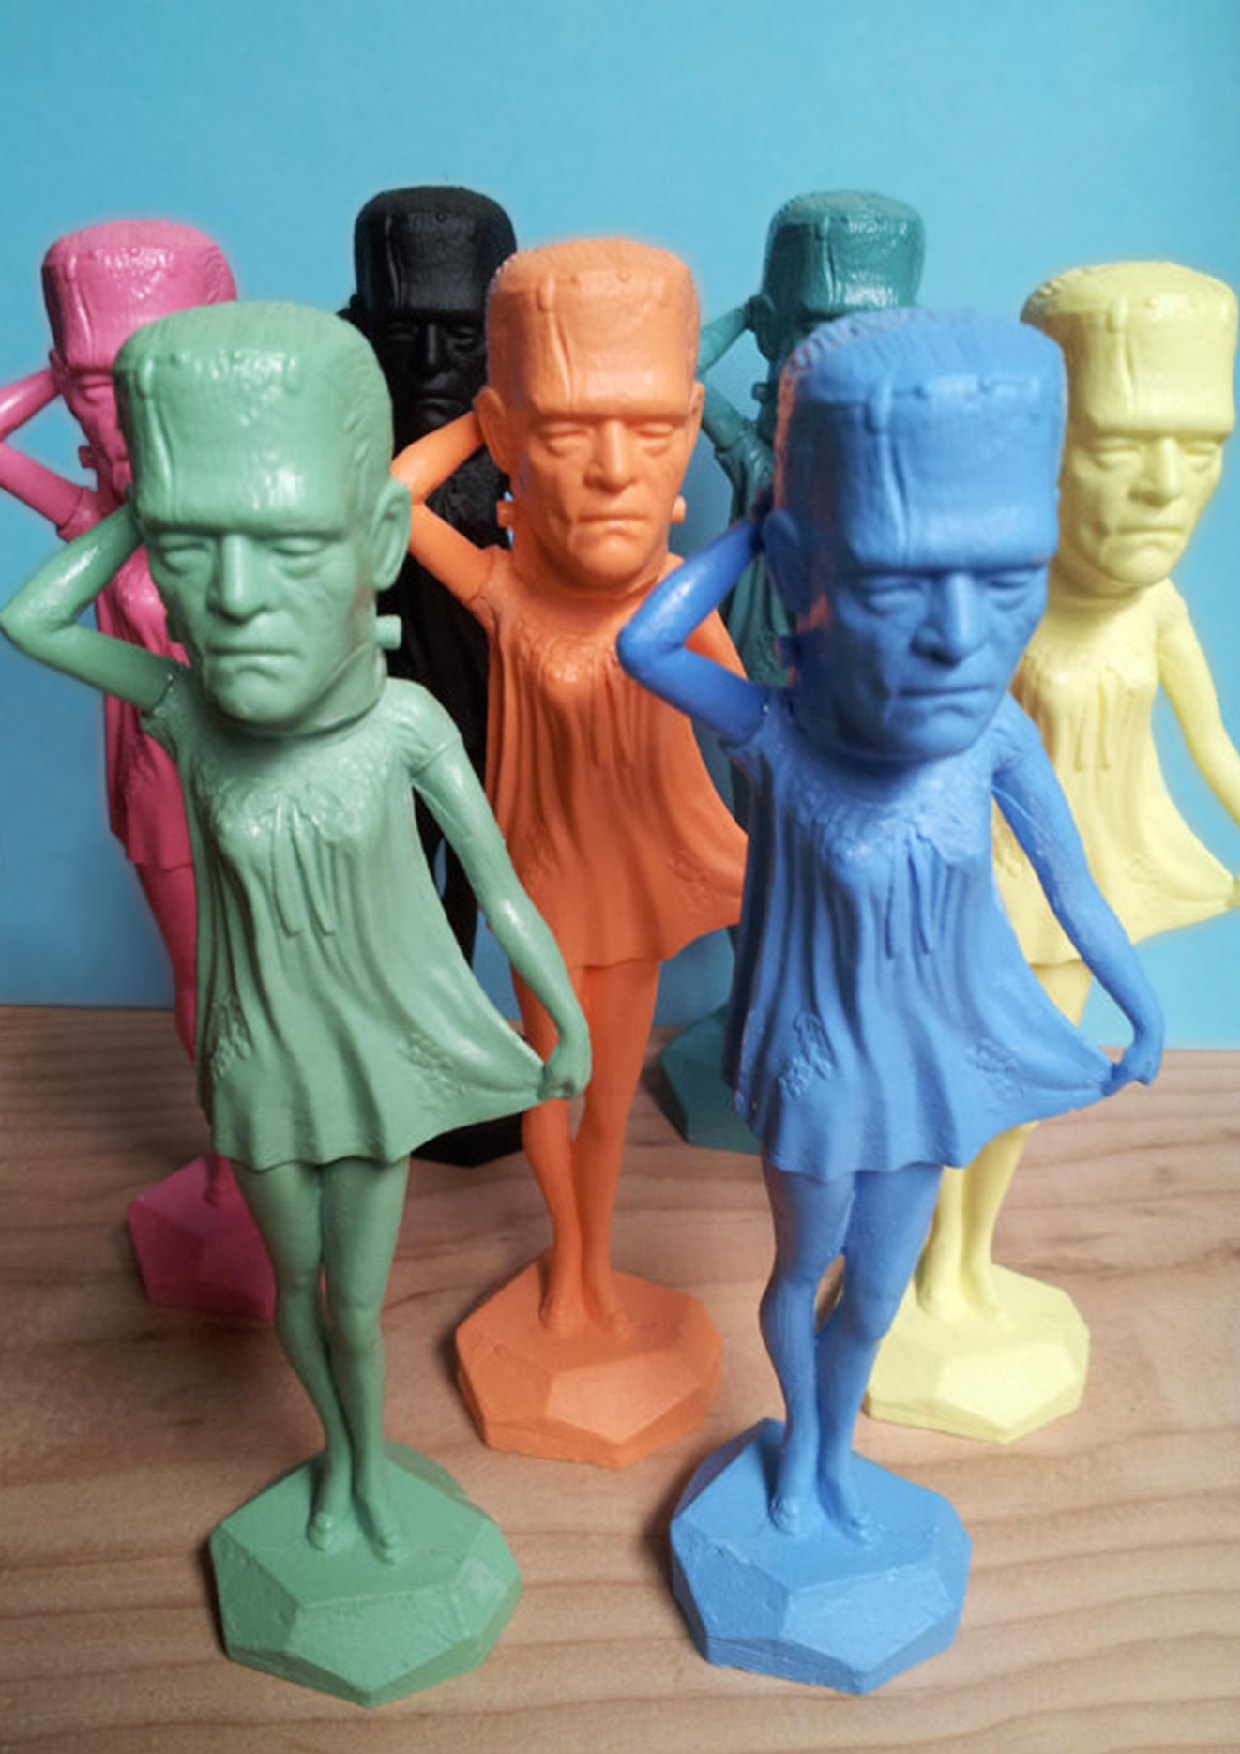
\includepdf{/Users/matthieulapeyre/Documents/phd_thesis/media/franki}


\chapter{Exploring the role of morphology with Poppy} % (fold)
\label{cha:exploring_the_role_of_morphology}


Poppy has been designed to be a new experimental platform opening the possibility to systematically study the role of morphology in sensorimotor control, in human-robot interaction and in cognitive development. Indeed, as we discussed in chapter REF, a suitable design of a robot morphology can greatly simplify control problems, increase robustness, and open new modes of interaction with the physical and social world. Thus, being able to study the body as an experimental variable, something which can be systematically changed and experimented, is of paramount importance. Yet, until recently it was complicated because building a robot relied on heavy and costly manufacturing techniques but 3D printing has changed the landscape of possible.

We introduced a design methodology relying on the use off-the-shell components, Arduino electronic architecture and in which the 3D printing has a central aspect for the production of mechanical part (see chapter~\ref{REF}).

Poppy transposes this methodology to humanoid robotics, and it is now possible to explore new body shapes in just a few days. In addition, its size, weight and power actuation highly reduce the risk of self-damage if a programming error occurs, which means experimentation can be directly conducted in the real world without having to either use physical simulator or build heavy experimental setup.

In this chapter, we present several experiments aiming to show by examples how the Poppy's morphology can be easily and quickly hacked for exploring morphological variants in the real world.
These experiments will be presented to show 4 differents

\begin{enumerate}
    \item Experimenting the role of morphology (section~\ref{sec:morphology-role})
    \item Adding new sensors on Poppy (section~\ref{sec:morphology-adding-sensors})
    \item Fast exploration of morphological variants (section~\ref{sec:morphology-variable})
    \item Adding a novel mechanism (section~\ref{sec:morphology-add-mechanism})
\end{enumerate}


% As an application of the methodology presented in the chapter REF, and especially interested by the role of morphology in the understanding of biped locomotion, we decided to use Poppy to explore the impact of particular leg design on bipedal stability.

% In this chapter, we suggest to explore the impact of the thigh shape on the lateral stability(see section~\ref{sec:experimental_thigh_shape}) and evaluate the efficient of foot designs for balance and biped locomotion.

% !TEX root = ../../thesis.tex

\newpage
\section{Experimental evaluation of the role of the morphology: the thigh shape} % (fold)
\label{sec:morphology-role}

The role of morphology in robot bipedal locomotion has been particularly explored through the research on passive dynamic walkers~\parencite{wisse2007passive}. The most famous example concerns Tad MacGeer's work~\parencite{mcgeer1990passive}. Thanks to the understanding of the intrinsic dynamics of its structure, McGeer has managed to create a 2D biped robot capable of producing several steps without any controller or motor.
The only control of this robot is obtained through the interaction between the intrinsic inertia of the structure and gravity.
This work has been pursued with the appearance of semi-passive walkers combining both specific passive properties and low power actuation to increase their robustness~\parencite{Anderson2005}. We can note the work of Collins~\parencite{collins2005bipedal} which explored the case of a semi-passive 3D biped robot. Its morphology is based on a particular mass distribution, knee locking, round feet and springs on the legs to generate an efficient walking gait while keeping its lateral and frontal balance.
The concept of the 3D semi-passive robot has been pushed even further with the realization of a complete humanoid robot with torso, arms and head: the robot Denise~\parencite{wisse2005three} and Flame presented in~\parencite{Hobbelen2008}.

\begin{figure}[!t]
\centering
    \subfloat[][bended thighs]{\label{fig:poppy_with_bended_legs}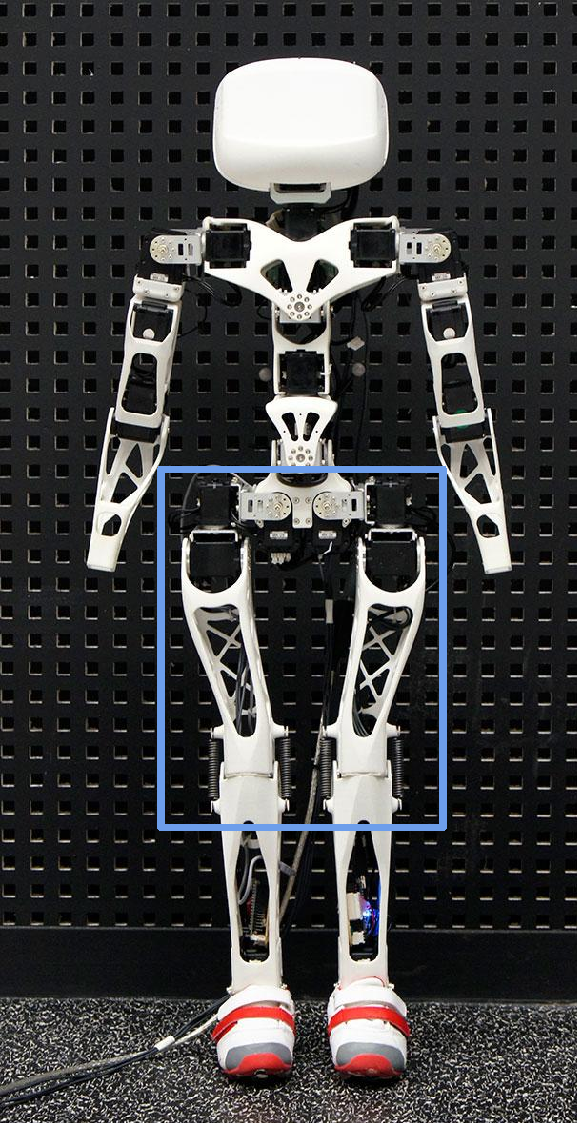
\includegraphics[width=0.35\linewidth]{poppy_bended_tigh_square.pdf}}
    \hfil
    \subfloat[][straight thighs]{\label{fig:poppy_with_classical_legs}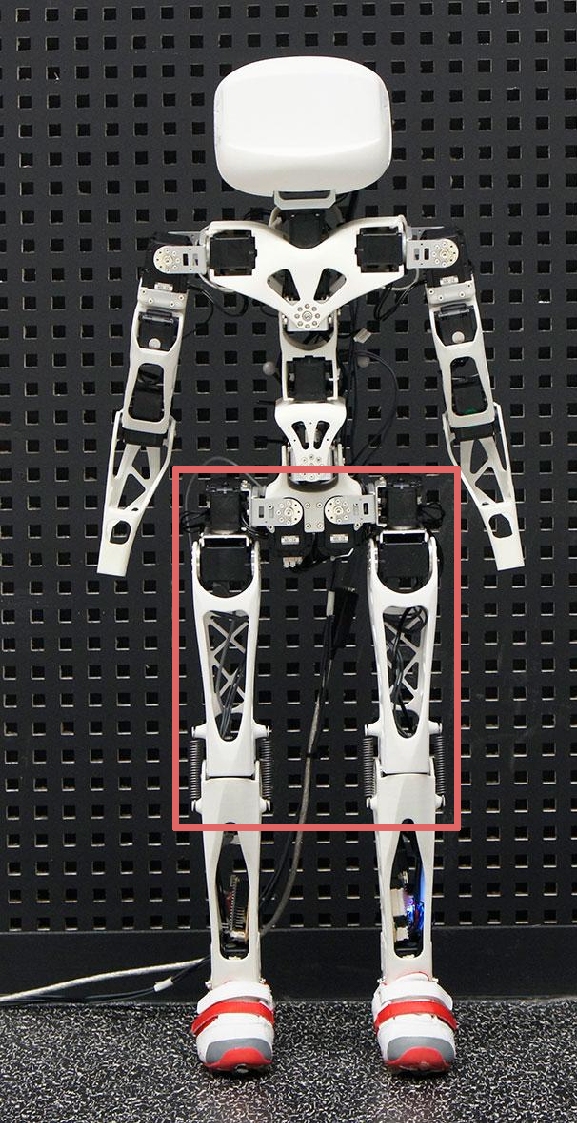
\includegraphics[width=0.35\linewidth]{poppy_straight_tigh_square.pdf}}
    \caption{We evaluate the effect of thigh morphology on the bipedal locomotion dynamic.
    Experiments are made using the Poppy humanoid platform.
    In this paper, we compare two thigh morphologies: (a) thigh bended by an angle of 6\textsuperscript{o} and (b) a more classical approach with straight thighs.}
    \label{fig:poppy_compared}
\end{figure}


The geometry and distribution of mass in the body has complex influences on bipedal locomotion. Several studies have for example, explored the role of the foot and ankle morphology for bipedal walking in both humans~\parencite{Adamczyk2006}~\parencite{Hughes1990} and robots~\parencite{hobbelen2005ankle}~\parencite{Davis2010}. However, to our best knowledge no research has focused on the role of the thigh for bipedal locomotion.  A few robots like HRP-4C~\parencite{kaneko2009cybernetic} and Kenshiro humanoid~\parencite{nakanishi2013design} robots seem to visually have a morphological design close to the thigh shape of Poppy, but no comparative study of the role of this shape was presented so far.

Thanks to the mechanical design of Poppy, allowing easy, cheap and fast morphological modifications, we are able to experiment with various thigh shapes on the robot’s dynamics and find out what impact those have. In particular, in this experiment, we will focus on its bio-inspired thigh shape, bended by an angle of 6\textsuperscript{o}. We will investigate the impact of this thigh design on balance and bipedal locomotion using a comparison with a more traditional straight thigh (see Fig.~\ref{fig:poppy_compared}).

% The results presented in the upcoming sections have been published in the Humanoids 2013 conference proceeding~\parencite{lapeyre:hal-00861110}.


\subsection{Understanding the role of the thigh shape in humans} % (fold)

If we look closely at the morphology of the human femur, it appears that it is inclined by an angle of 6\textsuperscript{o}. This makes the feet closer to the projection of the center of gravity (CoG) (see Fig.~\ref{fig:human_thigh}) therefore it reduces the distance traveled by the CoG to move from foot to another.

The model presented in appendix~\ref{appendix:thigh_model} has been used during the conception of Poppy to decide the use of bended thigh rather than classic straight one. This simple model, based on an inverted pendulum, shows this particular shape may enhance the stability in two main ways during the walking gait:

\begin{itemize}
    \item As the feet are closer to the center of gravity, the lateral translation of the CoG necessary to transfer the mass of the robot from one foot to another is reduced (see Fig~\ref{fig:human_thigh}). In the case of Poppy's morphology, thanks to the $6$\textsuperscript{o} bended thigh, the lateral motion of the CoG is reduced by about 30\% ($ 5 cm$ instead of $7.1 cm$).
    \item During the stance phase, the CoG initial conditions are slightly modified. Therefore it reduces the CoG falling speed at the begining. So if we consider the first 700 ms of the system behavior simulation and compare the two systems, the mean of the CoG falling speed is reduced by around 56\% in the bended thigh case.
\end{itemize}


\begin{figure}[tb]
\centering
    \subfloat[][]{\label{fig:human_thigh}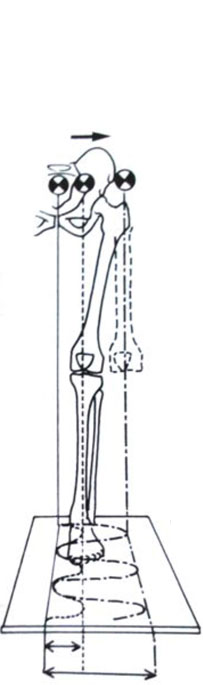
\includegraphics[height=8cm]{human_thigh.jpg}}
    \hfil
    \subfloat[][]{\label{fig:thigh_of_poppy}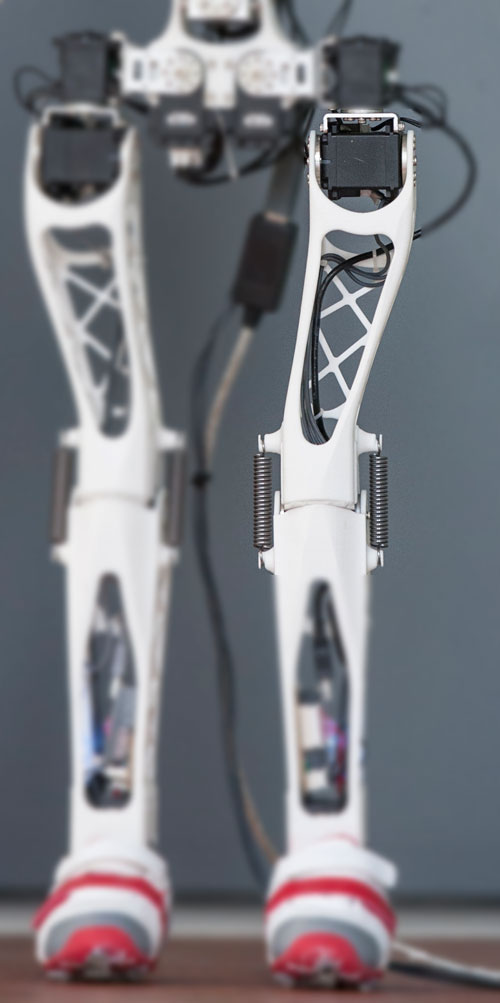
\includegraphics[height=6cm]{thigh_shape_large.jpg}}
    \caption{ a) Effect of bended human femur on human bipedal locomotion.
    c) Implementation of the bended thigh on the poppy platform}
    \label{fig:poppy_thigh}
\end{figure}

\subsection{Experimenting with variable thigh properties on Poppy} % (fold)

The simple model described in appendix~\ref{appendix:thigh_model} showed that a slight inclination (6\textsuperscript{o}) of the thigh can theoretically achieve a significant gain in the lateral stability of the robot during the two main phases of the walking gait (i.e. single stance phase and double stance phase).
Yet this model is very simple and Poppy allows to experiments easily the role of morphology in the real world with all its complexity.

Therefore we modified the thigh shape and printed it. As shown on the \figurename~\ref{fig:thigh_drawings}, the only modified paramater is the thigh bending angle, two cases: 6\textsuperscript{o} and 0\textsuperscript{o}.

\begin{figure}[p]
    \begin{center}
        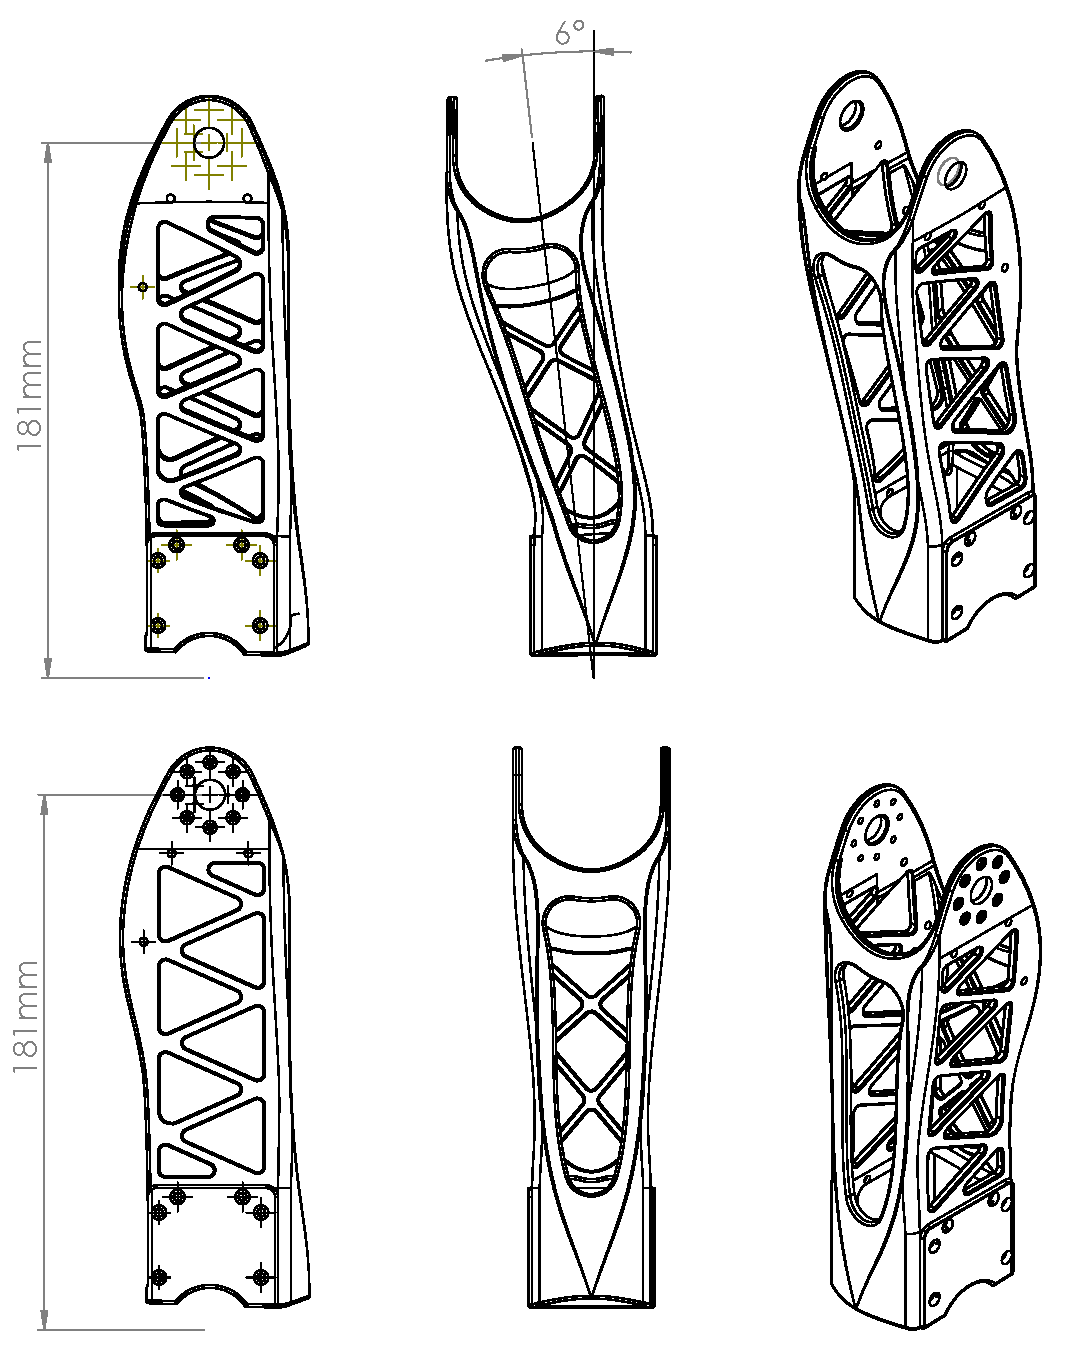
\includegraphics[height=\linewidth]{thigh_morpho.pdf}
    \end{center}
    \caption{Caption here}
    \label{fig:thigh_drawings}
\end{figure}

In this section, we describe representative experiments which evaluate the actual gain of the thigh shape on the real Poppy platform. To do this, we used both a pair of straight thighs and the bended thighs presented above. We will compare Poppy's reactions with those different legs (see \figurename~\ref{fig:poppy_compared} and \figurename~\ref{fig:thigh_drawings}) on three experiments:
\begin{itemize}
    \item Evaluate the falling speed during single support stance.
    \item Measure the lateral translation to move the CoG Form one foot to the other.
    \item Record the upper body motion during bipedal locomotion.
\end{itemize}

\subsubsection{Single support falling velocity} % (fold)
\label{ssub:falling_velocity}
The experiment evaluates the velocity of fall  when Poppy  is supported on only one foot and compare it with the theoretical results obtained in~\ref{sub:exp_theoritical_model}. To do so, the robot's head is tracked by an Optitrack\footnote{\url{http://www.naturalpoint.com/optitrack/products/v120-trio/}} device and markers are placed on the head. In postural balance on two feet, a motor order triggers the raise of a foot which unbalances the robot (see Fig.~\ref{fig:falling_experiment_dispositif}) and causes its lateral fall (see Fig.~\ref{fig:fall_of_poppy}). This experiment was repeated about fifteen times for the two cases studied, i.e. with bended legs (Fig.~\ref{fig:poppy_with_bended_legs}) and with straight legs (Fig.~\ref{fig:poppy_with_classical_legs}).

\begin{figure}[h]
\centering
    \subfloat[][]{\label{fig:falling_experiment_dispositif}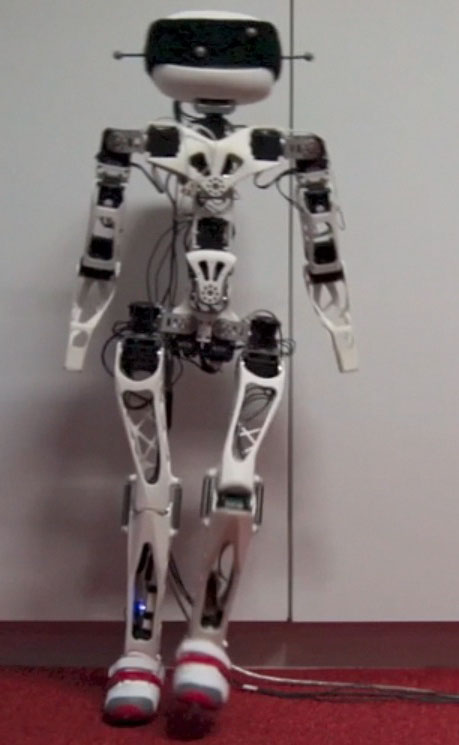
\includegraphics[height=6cm]{experience_fall_illu.jpg}}
    \hfil
    \subfloat[][]{\label{fig:fall_of_poppy}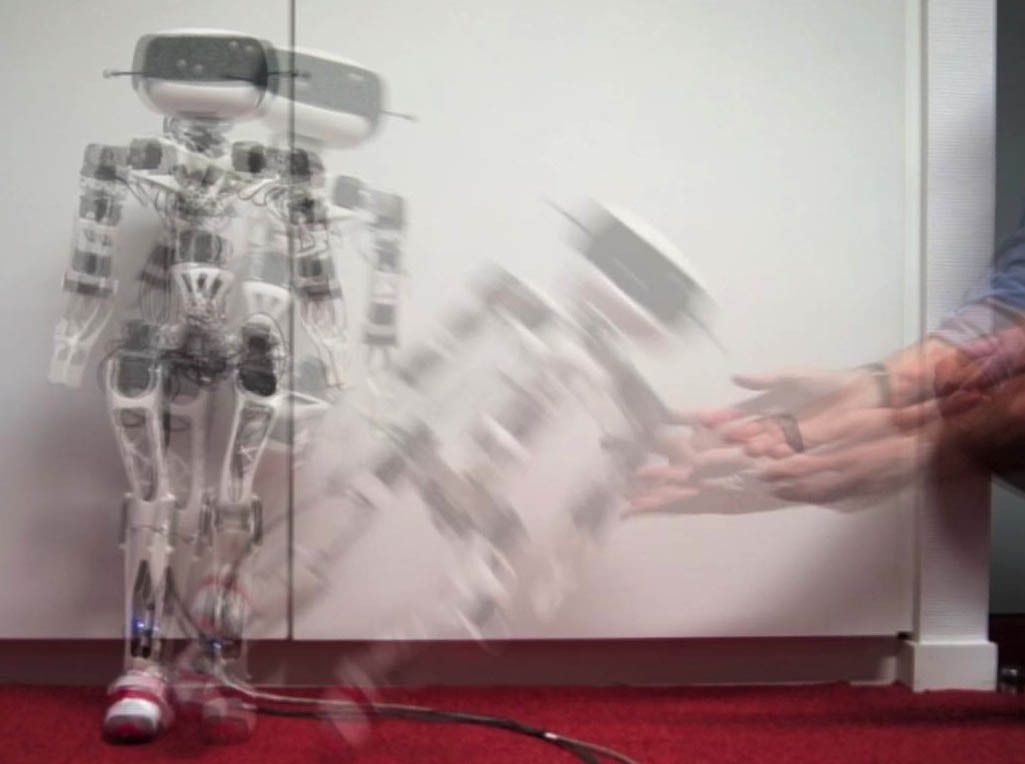
\includegraphics[height=6cm]{experience_fall_mean.jpg}}
    \caption{Run of the single support falling experiment.
    The markers on Poppy’s headband track its absolute position over time.
     a) Initial perturbation provoked by the sudden raise of one foot, b) view of Poppy’s lateral fall over time.}
    \label{fig:falling_experiment}
\end{figure}

Experimenta results are shown in Fig.~\ref{fig:falling_results}. The blue color is assigned to experiments with bended thighs while the red color is assigned to straight thighs. For each case, the light color corresponds to the standard deviation and the dark color to the 95\% confidence interval of the mean value. The first figure~(\ref{fig:fall_result_position}) refers to the head altitude position over time and the second~(\ref{fig:fall_result_velocity}) to the falling velocity of the head. Dashed lines represent theoretical results obtained with the model presented in section~\ref{fig:model_thigh}. We notice the strong similarity both on the shape and on the difference between the two morphologies studied. Yet, there is a slight time shift between theoretical and experimental results. This can be explained by the inertia of the real robot which was not taken into account during the simulation.

\begin{figure}[h]
\centering
    \subfloat[][Vertical head position]{\label{fig:fall_result_position}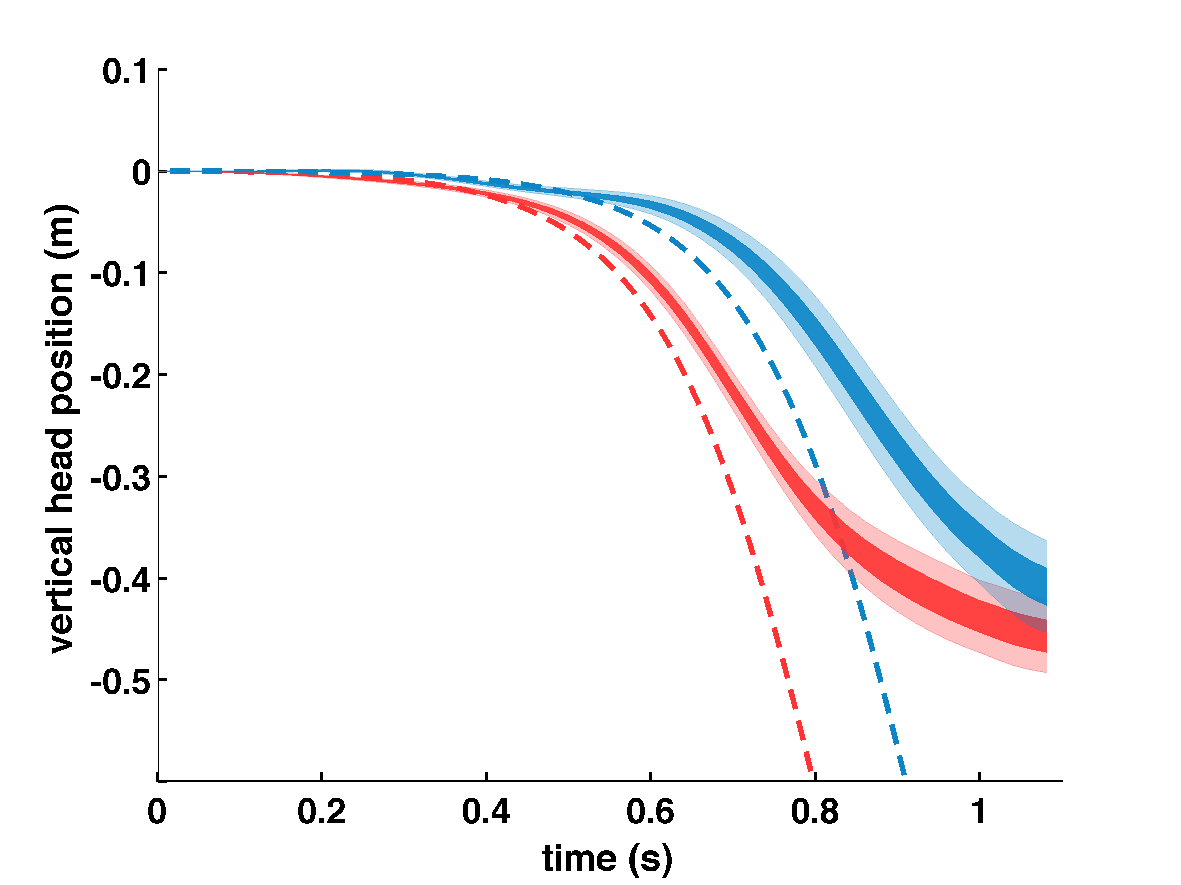
\includegraphics[width=0.50\linewidth]{falling_compare.pdf}}
    \hfil
    \subfloat[][Vertical head falling velocity]{\label{fig:fall_result_velocity}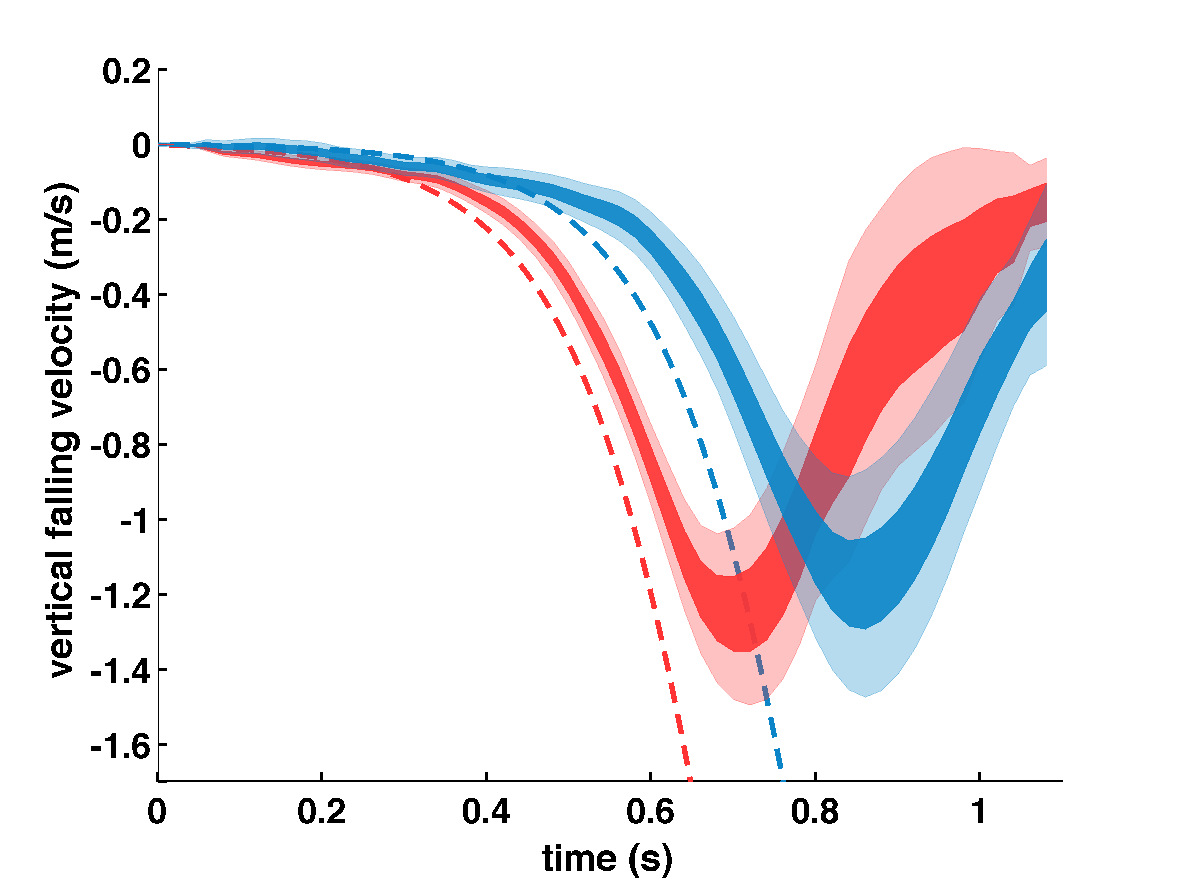
\includegraphics[width=0.50\linewidth]{velocity_compare.pdf}}
    \caption{Results of the single support falling experiment.
    The blue color is associated with experiments conducted with bended thighs while the red color is assigned to straight thighs.
    For each case, the light color corresponds to the standard deviation and the dark color to the 95\% confidence interval of the mean value while dashed lines represent theoretical results.
    These figures show the vertical position (a) and vertical falling velocity (b) of the head of Poppy over time for each case studied.
    The curve’s behavior change after 800 min is due to the fact that we catch the robot before it touches the ground.}
    \label{fig:falling_results}
\end{figure}

These figures show a clear improvement for the version of Poppy with bended thighs (blue curves) with a 200 min time shift compared to the straight thighs (as illustrated on the attached video\footnote{\url{http://flowers.inria.fr/Humanoid2013/}\label{video}}).
Thanks to this delay, the falling speed is reduced by about 56\% during the first 700ms. Thus the robot remains almost stationary for 600 min (400 min in the case of straight thigh).  Poppy’s typical walking gait  takes a period of one second so the mono-pedal stance phase lasts around 420 min~\parencite{lapeyre2013poppy}. Considering that the robot remains stationary during more time than the single stance phase, we can imagine that the lateral balance control will be reduced during the walking gait.



\subsubsection{Double support CoG transfer} % (fold)
\label{sub:cog_motion}


In this experiment we evaluate the lateral movement of the robot necessary to cause a displacement of its center of gravity from one foot to the other and we verify the theoretical results obtained previously. For this, Poppy is placed on a force platform to measure the displacement of its center of pressure. The absolute movements of the robot are tracked with an OptiTrack device and markers placed at the head and lower back (approximately the position of the actual center of gravity). The robot is kept rigid in a neutral position and a human physically pushed it from left to right until it reached its lateral falling limit. As this operation is not very accurate, the experiment is repeated one hundred times.

\begin{table}[h]
\centering
\begin{tabular}{|l|c|c|c|}
  \hline &      Straight tigh &                     Bended Tigh &                   diff(\%) \\
  \hline CoP & 74.6 {\scriptsize$\pm$9.0} mm &     49.8 {\scriptsize$\pm$7.7} mm & 33\\
  Head & 100.1{\scriptsize$\pm$14.4} mm&     62.9{\scriptsize$\pm$22.0} mm &  37\\
  Lower Back & 64.1{\scriptsize$\pm$11.5} mm&      43.4{\scriptsize$\pm$15.0} mm &  32 \\
  \hline
\end{tabular}
\caption{Summary of the results obtained during the experiment on the lateral motion needed to transfer the robot’s mass from one foot to the other.}
\label{tab:CoG_motion}
\end{table}

Table~\ref{tab:CoG_motion} presents for each area considered (i.e. center of pressure (under feet), lower back and head motion) the amplitude of the lateral motion (in millimeters) needed to translate the CoG of the robot from one foot to the other for the two versions of Poppy’s thigh design. The last columns summarize the relative difference between the two conceptions (in percent). One can note that the results show a reduction of lateral movement of around 30\%. Thanks to the shape of the thigh, the lateral displacement of the upper body required to move the CoG from one foot to the other can be reduced.


The results presented on the two first experiments show improvement for two main aspects needed during bipedal locomotion: lateral stability and mass transfer. In the next experiment, we will evaluate if there is a significant performance gain in a complex dynamic phase such as bipedal walking.


\subsubsection{Walking dynamic} % (fold)
\label{sub:walking_dynamic}

As explained in the introduction and description of the platform, Poppy has been specially designed to study bipedal walking and human-robot interaction.

Here the experiment consists of playing an open-loop walking pattern while the robot is guided through the physical interaction with a human. The user’s role is to provide both balance and control of mass transfer. By producing small lateral motion on the upper-body they can help the robot to move its CoG from one foot to another.

\begin{figure}[tb]
    \centering
    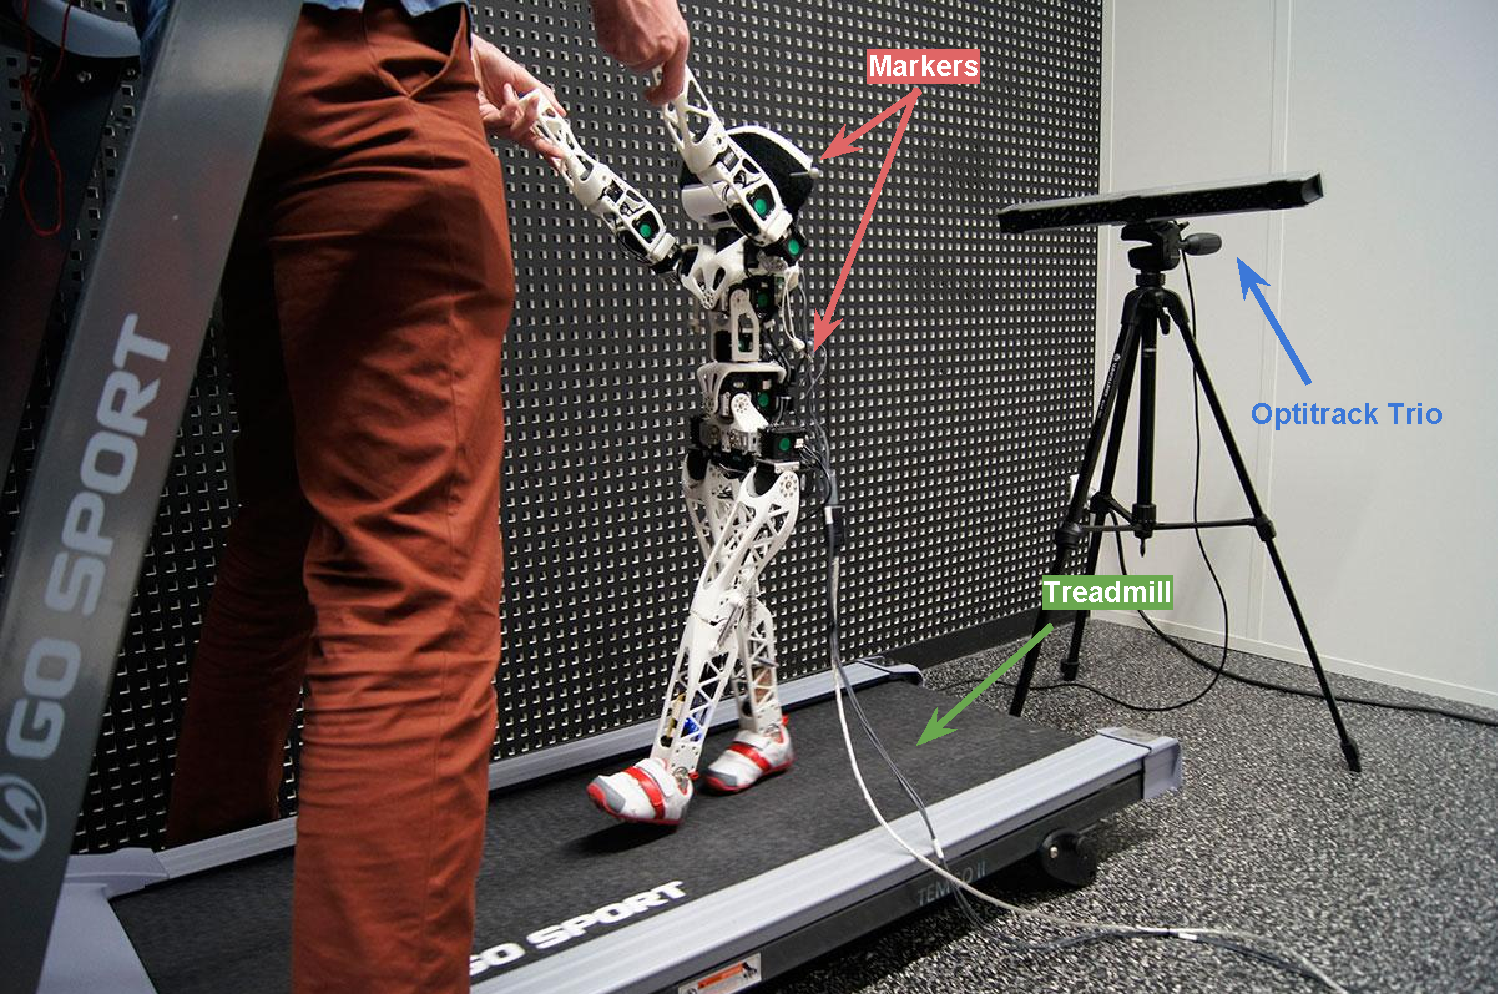
\includegraphics[width=0.8\linewidth]{dispositif_experience_marche.pdf}
    \caption{Proceeding of the walking experiment.
    Poppy is tracked by an Optitrack trio while it is walking on a treadmill set at 1.8km/h.
    An expert user provides the sagittal balance needed throughout the experiment.}
    \label{fig:walking_experiment}
\end{figure}


The gait is based on the actual human sagittal joint kinematic~\parencite{Nester2003}: hip, knee, ankle (see Fig.~\ref{fig:CPG}.a). A direct transposition of the human joint kinematic on the Poppy's morphology results in a walking speed which is too fast to be handled by users (see Fig.~\ref{fig:CPG}.b). A simple reduction of a joint’s amplitude leads to an unsuitable leg trajectory where toes bump into the ground during the swing phase (see Fig.~\ref{fig:CPG}.c). So to ensure enough clearance during the swing phase and suitable walking speed for the guidance with a user, we modified the trajectories of the joints by hand to both reduce the length step and increase the foot clearance (see Fig.~\ref{fig:CPG}.d). The actual gait on Poppy is shown in Fig.~\ref{fig:humanoids2013_cpg_on_poppy}.


\begin{figure}[tb]
    \centering
    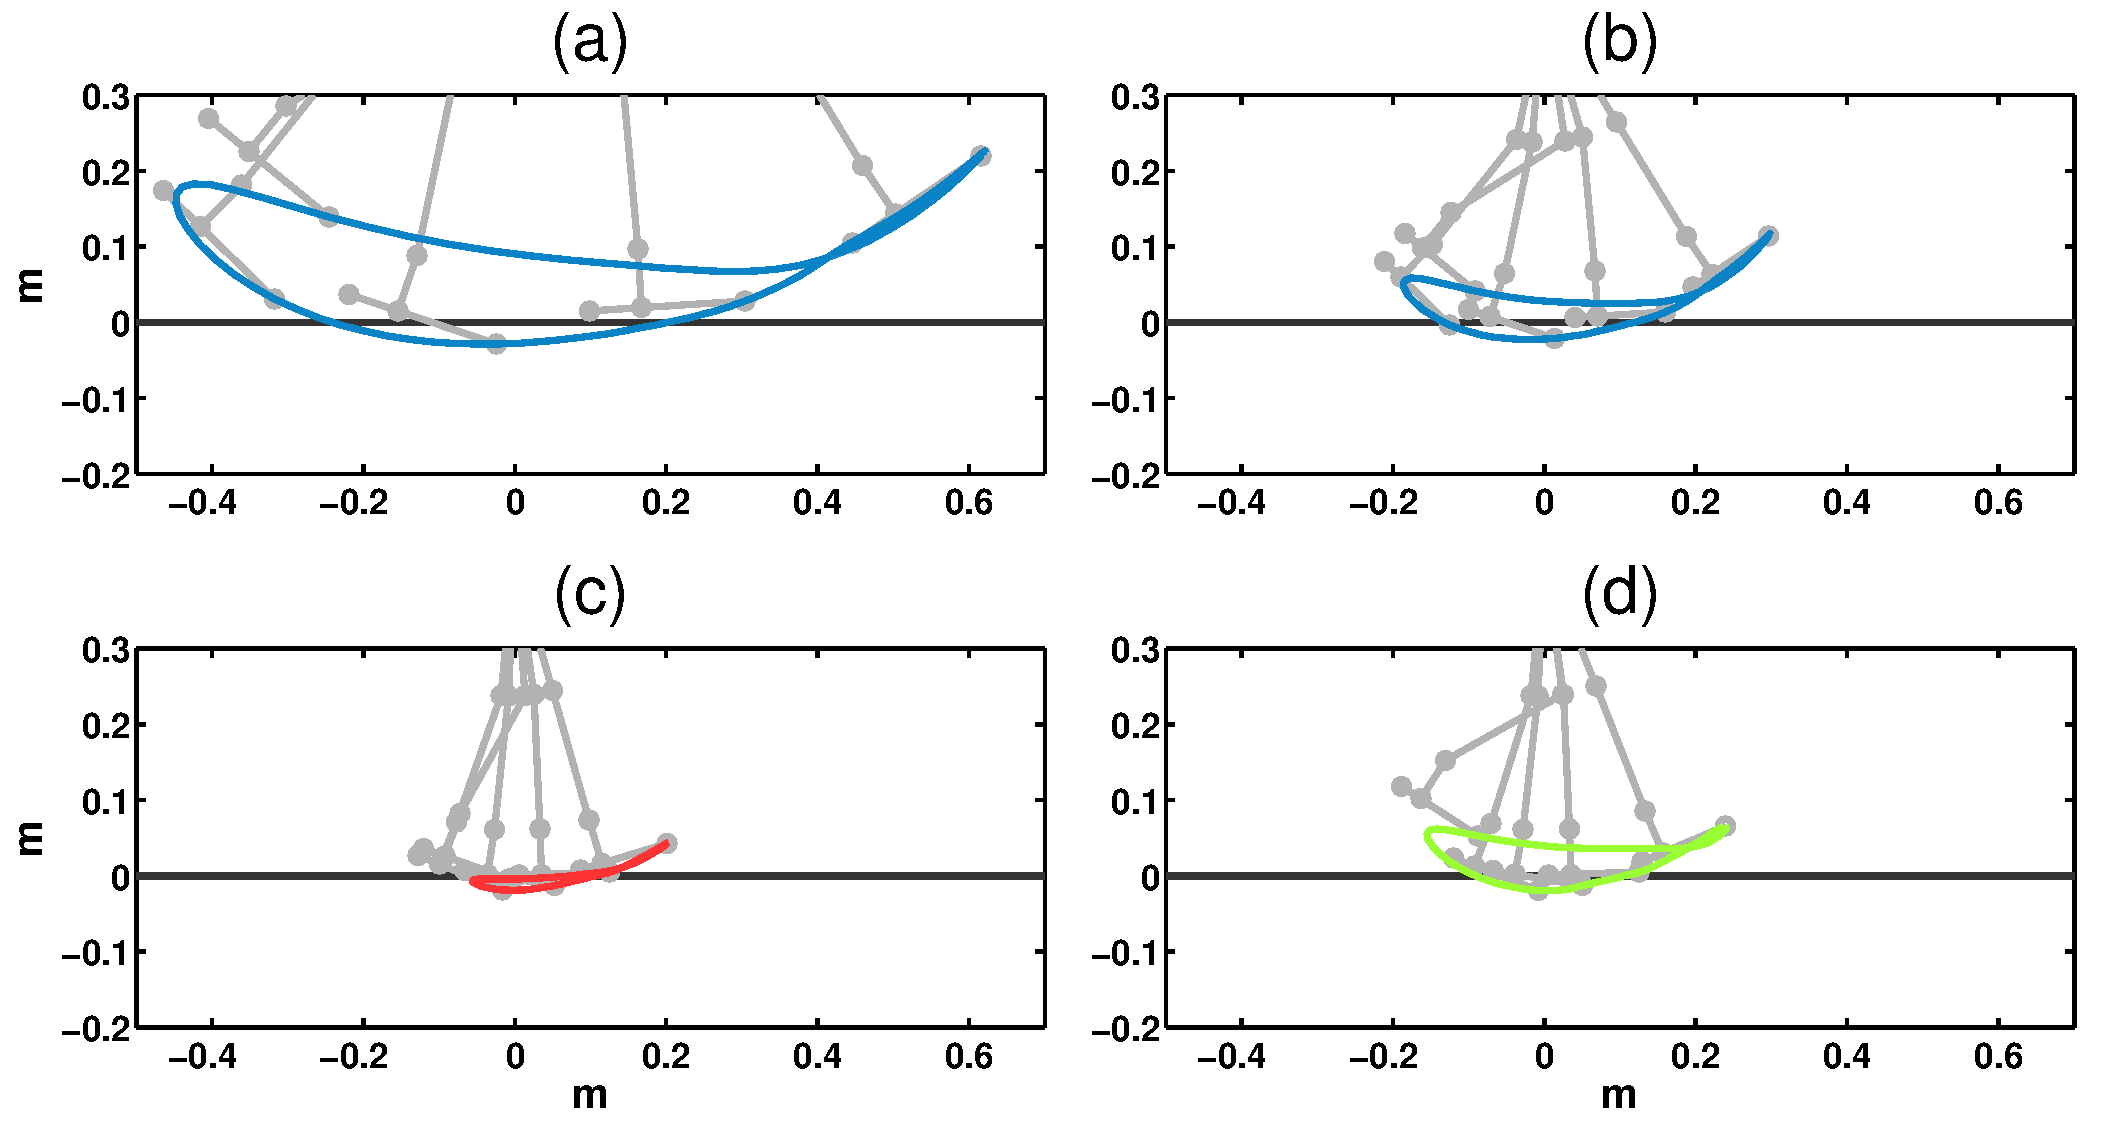
\includegraphics[width=0.95\linewidth]{CPG.pdf}
    \caption{Trajectories of toes generated by the walking pattern a) Kinematics of human walking
    with human morphology b) Direct transposition of human kinematics onto Poppy's morphology
    c) Reducing amplitude of the human kinematics joints with Poppy's morphology d) Walking pattern
    used for the experiment with Poppy}
    \label{fig:CPG}
\end{figure}

\begin{figure}[tb]
    \centering
    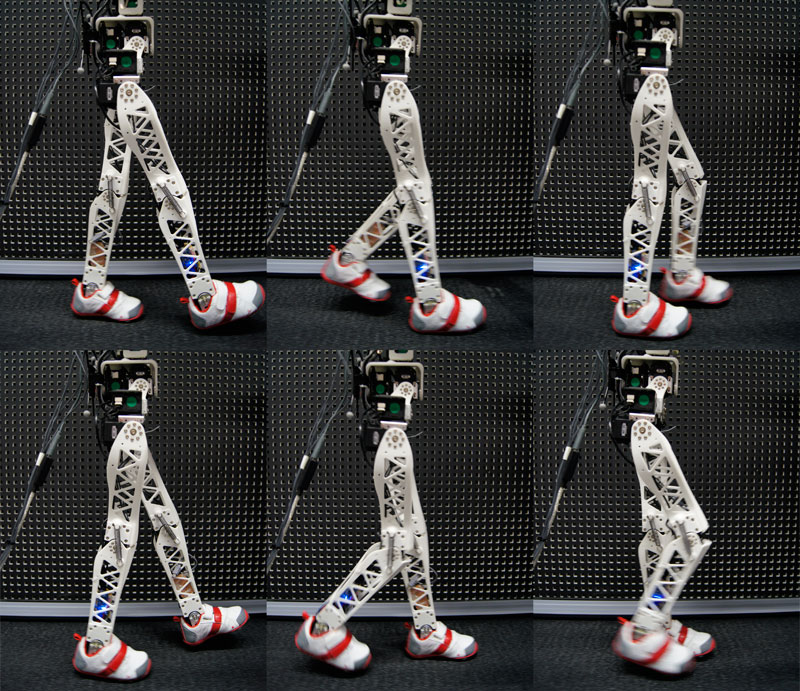
\includegraphics[width=0.7\linewidth]{walking_poppy.jpg}
    \caption{Walking gait CPG described on Fig.~\ref{fig:CPG}.d applied on the actual Poppy robot.
    The CPG generates a human-like walking gait allowing the robot to walk at 1.8km/h and involves straight legs during the stance phase.
    There is no balance control but stability is obtained through physical guidance with a trained expert user.}
    \label{fig:humanoids2013_cpg_on_poppy}
\end{figure}

In this experiment we are interested in the dynamic of Poppy especially on the frontal plane and we will compare the effect of the thigh shape on this dynamic. Poppy walks on a treadmill following the walking gait described above. An expert user trained to keep the robot in the correct walking cycle provides guidance to the robot. This is done by keeping the robot in a vertical position and supporting, in a compliant manner, the lateral movement of the robot as illustrated in attached videos. The user is asked to do the best he can to minimize the movement/forces he applies in both morphologies to reduce the bias towards the two designs experimented. All proprioceptive sensors are recorded at 50hz while an Optitrack device associated  with markers located at the head and lower back measure the absolute displacements of the robot (voir Fig.~\ref{fig:walking_experiment}).



Poppy’s movement is recorded for around 1800 walking gait cycles for each thigh design (around 90,000 data points for each case). Data are folded over to extract the gait behavior over a gait cycle. Results are presented in Fig.~\ref{fig:walk_result}. As previously, the blue color is assigned to experiments with bended thighs, the red color is assigned to straight thighs. For each case, the light color corresponds to the standard deviation and the dark color to the 95\% confidence interval of the mean value.

\begin{figure}[p]
    \subfloat[][Lateral head displacement]{\label{fig:head_position}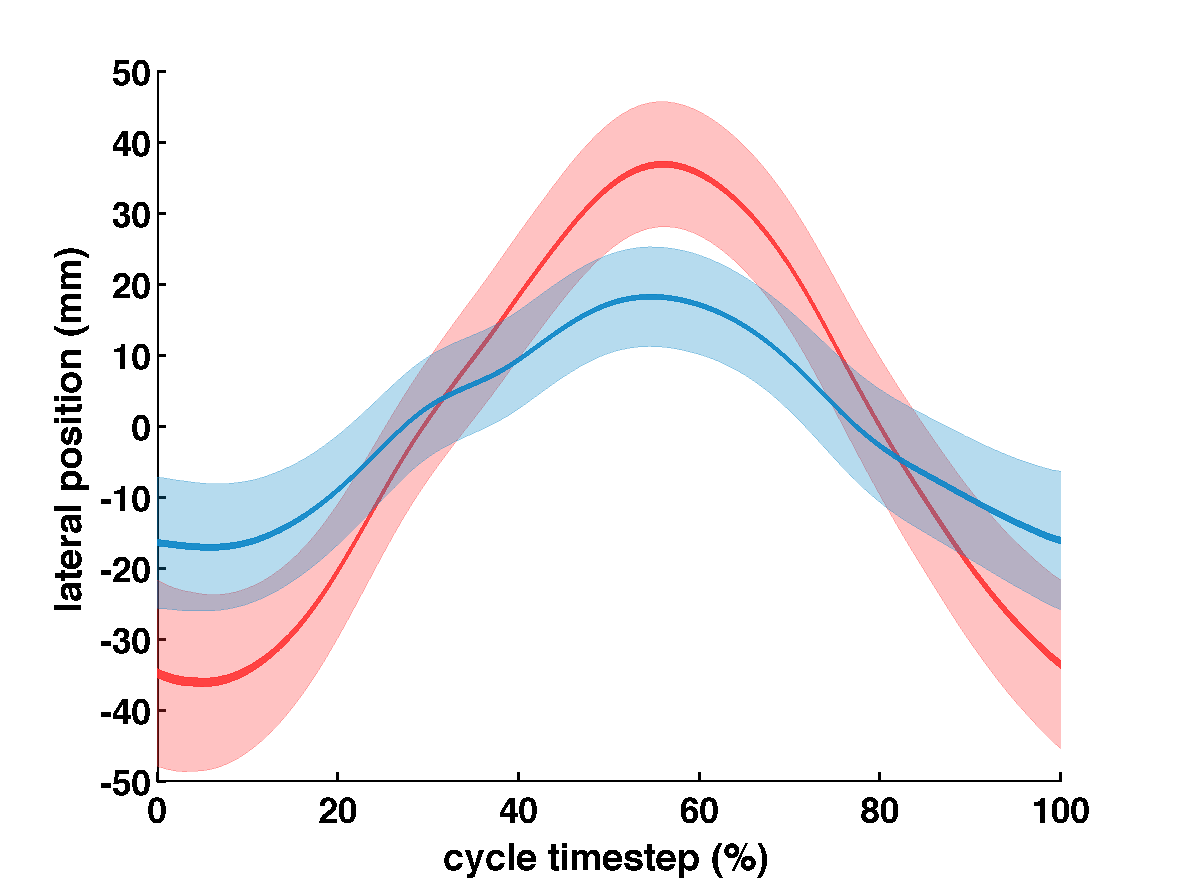
\includegraphics[width=0.49\linewidth]{marche_head_motion.pdf}}
    \hfil
    \subfloat[][Lateral lower back displacement]{\label{fig:low_back_position}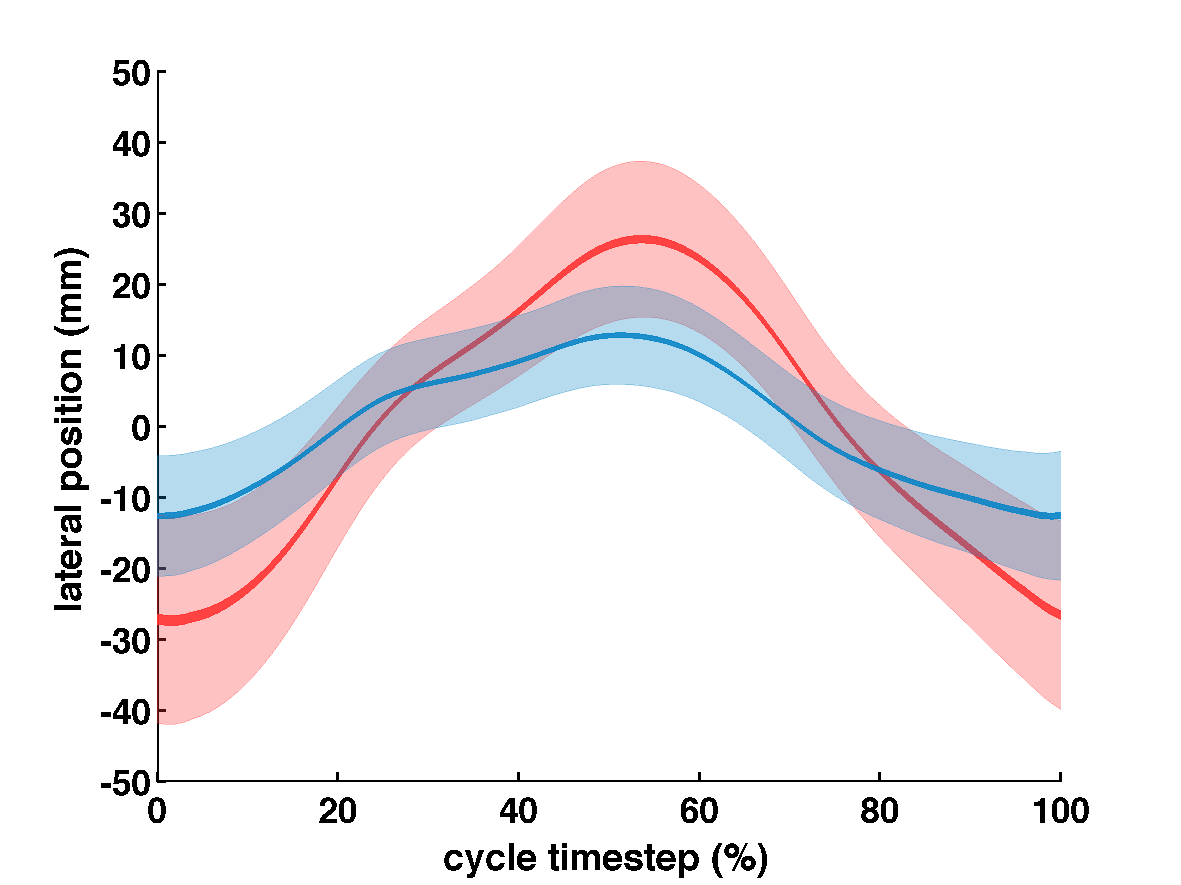
\includegraphics[width=0.49\linewidth]{marche_low_back_motion.pdf}}
    \hfil
    \subfloat[][Sagittal head acceleration]{\label{fig:head_acceleration_x}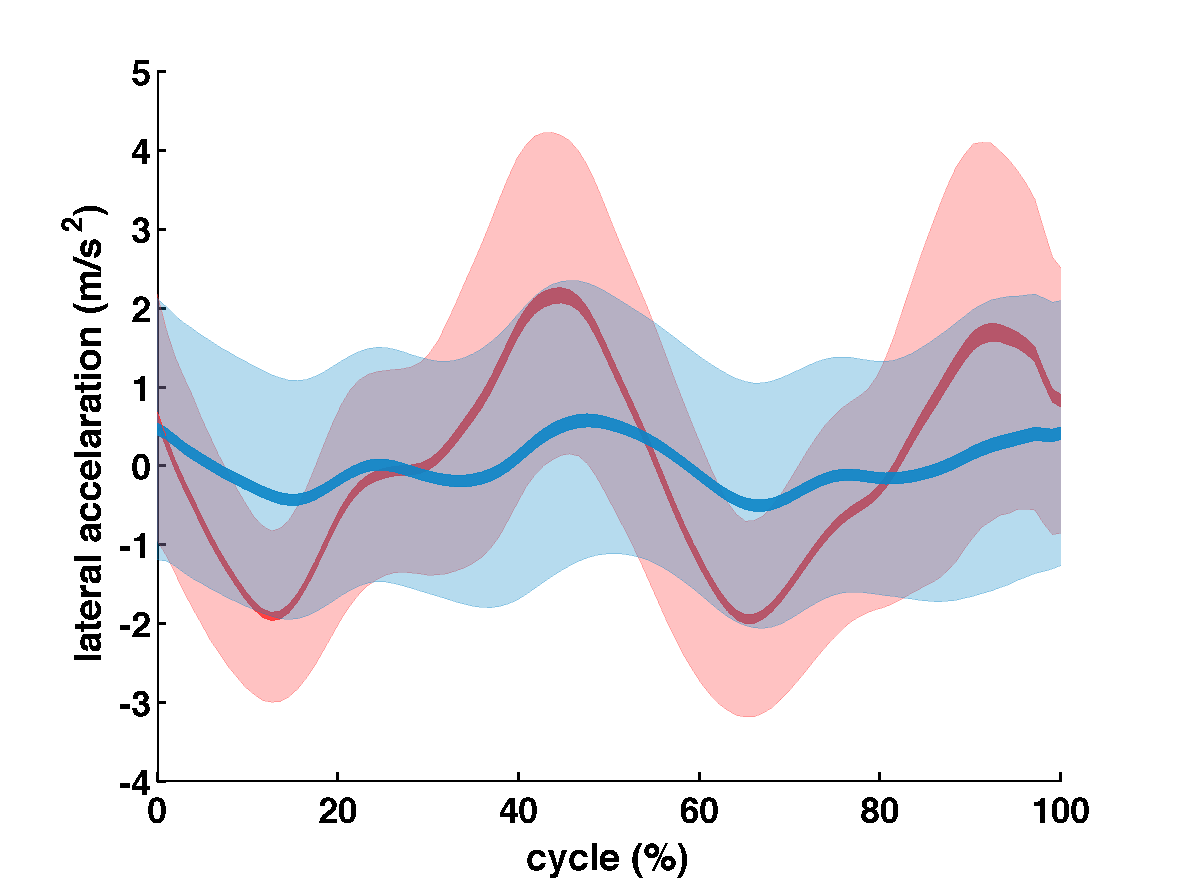
\includegraphics[width=0.49\linewidth]{marche_accel_x_signal.pdf}}
    \hfil
    \subfloat[][Lateral head acceleration]{\label{fig:head_acceleration_y}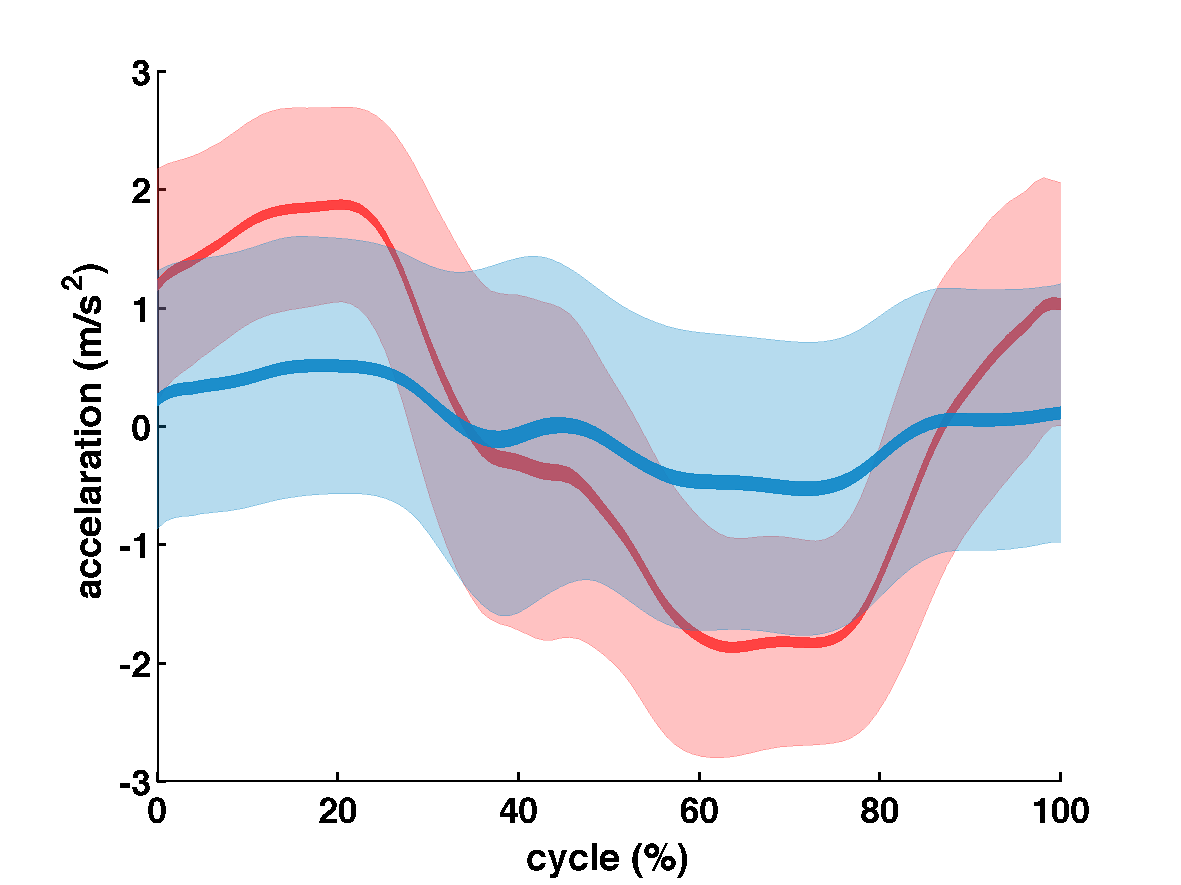
\includegraphics[width=0.49\linewidth]{marche_accel_y_signal.pdf}}
    \hfil
    \subfloat[][Speed of rotation in the frontal plane]{\label{fig:head_gyro_x}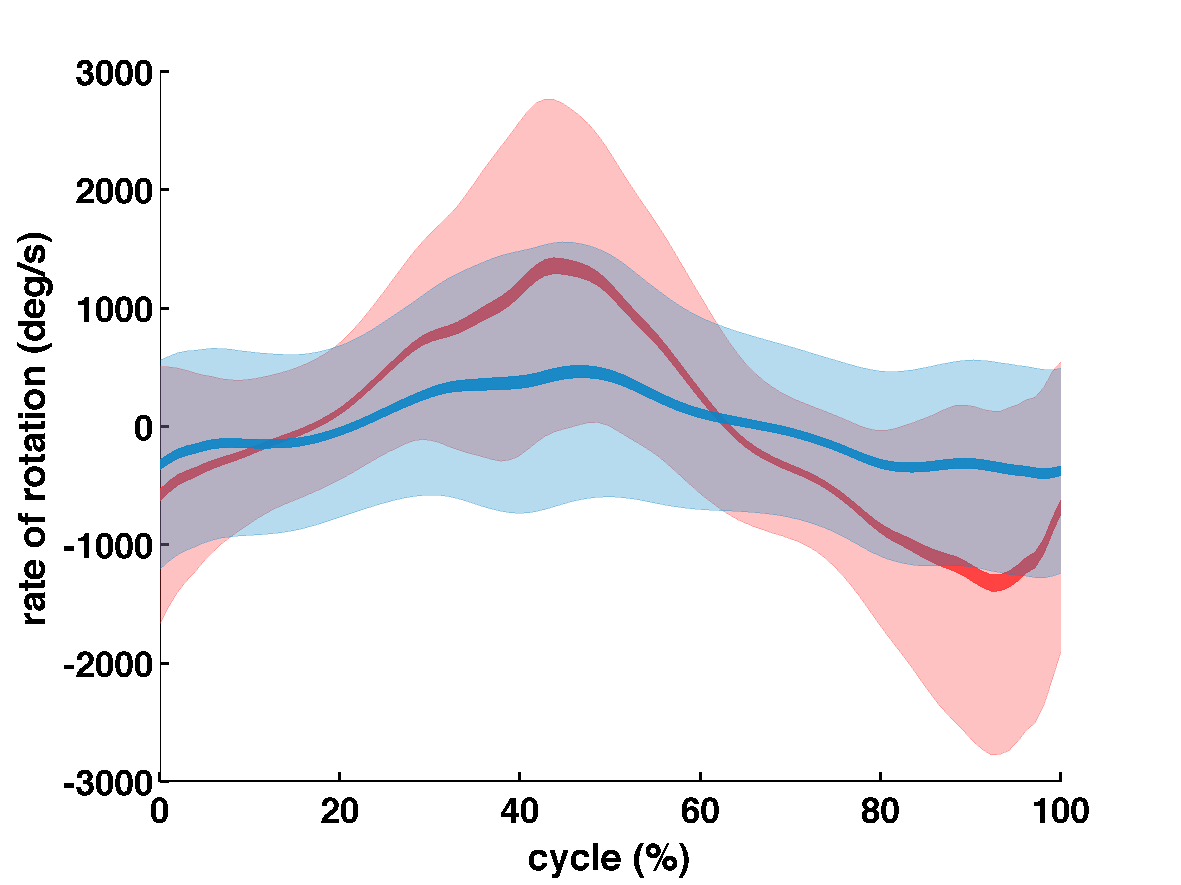
\includegraphics[width=0.49\linewidth]{marche_tilt_x_signal.pdf}}
    \hfil
    \subfloat[][Head inclinaison]{\label{fig:head_tilt_x}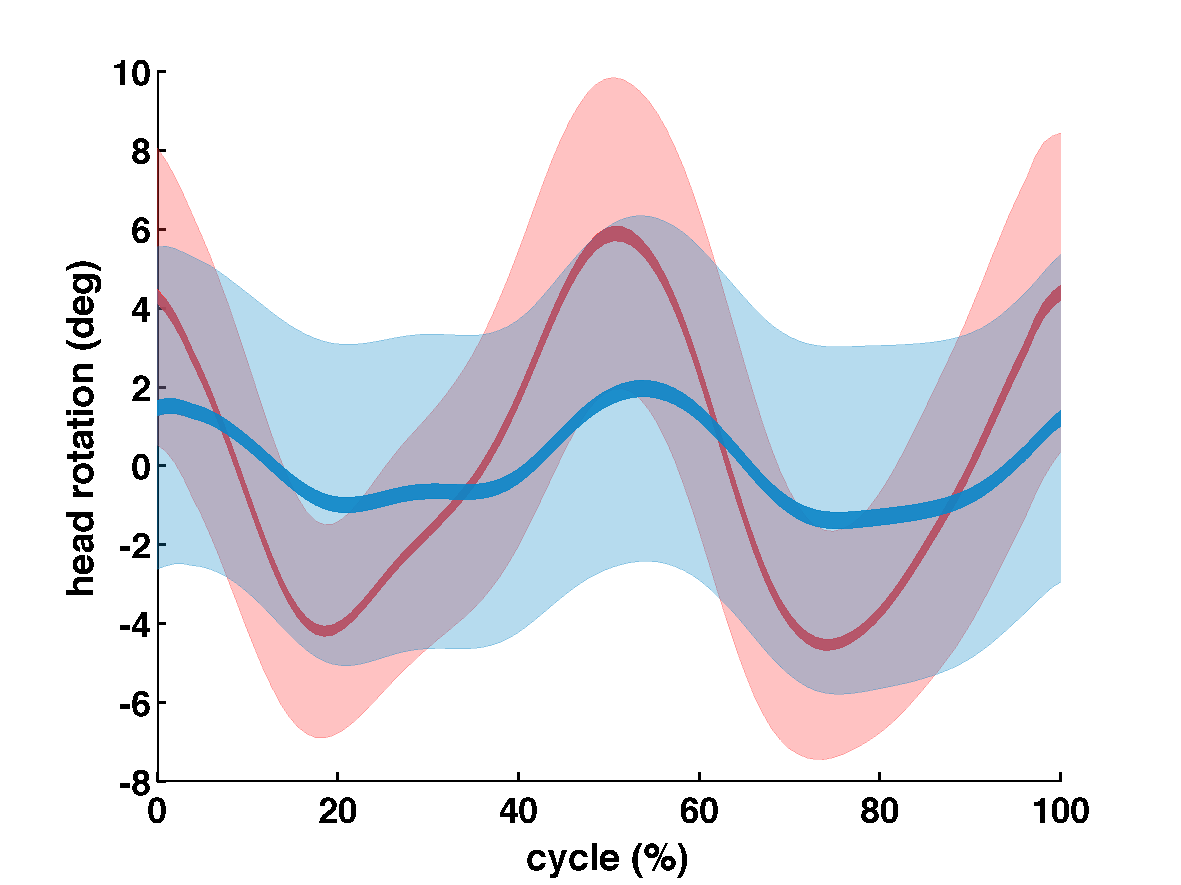
\includegraphics[width=0.49\linewidth]{marche_tilt_y_signal.pdf}}
    \caption{Results obtained during the walking experiment.
    The blue color is associated with experiments conducted with bended thighs while the red color is assigned to straight thighs.
    For each case, the light color corresponds to the standard deviation and the dark color to the 95\% confidence interval of the mean value.
    All data are folded over to extract the mean gait behavior and its standard deviation over a walking gait cycle expressed in percent.}
    \label{fig:walk_result}
\end{figure}

The two first figures (i.e. ~\ref{fig:head_position} and ~\ref{fig:low_back_position}) show the lateral motion of the upper body in millimeters over the gait cycle. We notice that for the two designs, the motion pattern shown by the upper body (head and lower back) is similar. However, in the case of the bended thigh (blue) the amplitude of the motion is reduced by about 45\%. Another interesting effect concerns the head perturbations shown on figures ~\ref{fig:head_acceleration_x}, and ~\ref{fig:head_acceleration_y}. Here also, patterns are similar but in the case of the bended thigh the head is clearly less perturbed by the walking dynamic, with a reduction in amplitude of approximately 30\%. Five pictures were taken while Poppy was walking and were stacked in Fig.~\ref{fig:poppy_walking_compared}. This shows a qualitative point of view of the walking dynamic for both studied cases.
We notice that the lateral motion of the version of Poppy with bended thighs~\ref{fig:poppy_walking_bended} is small compared to the version with straight thighs~\ref{fig:poppy_walking_straight}.


\begin{figure}[h]
\centering
    \subfloat[][bended thigh]{\label{fig:poppy_walking_bended}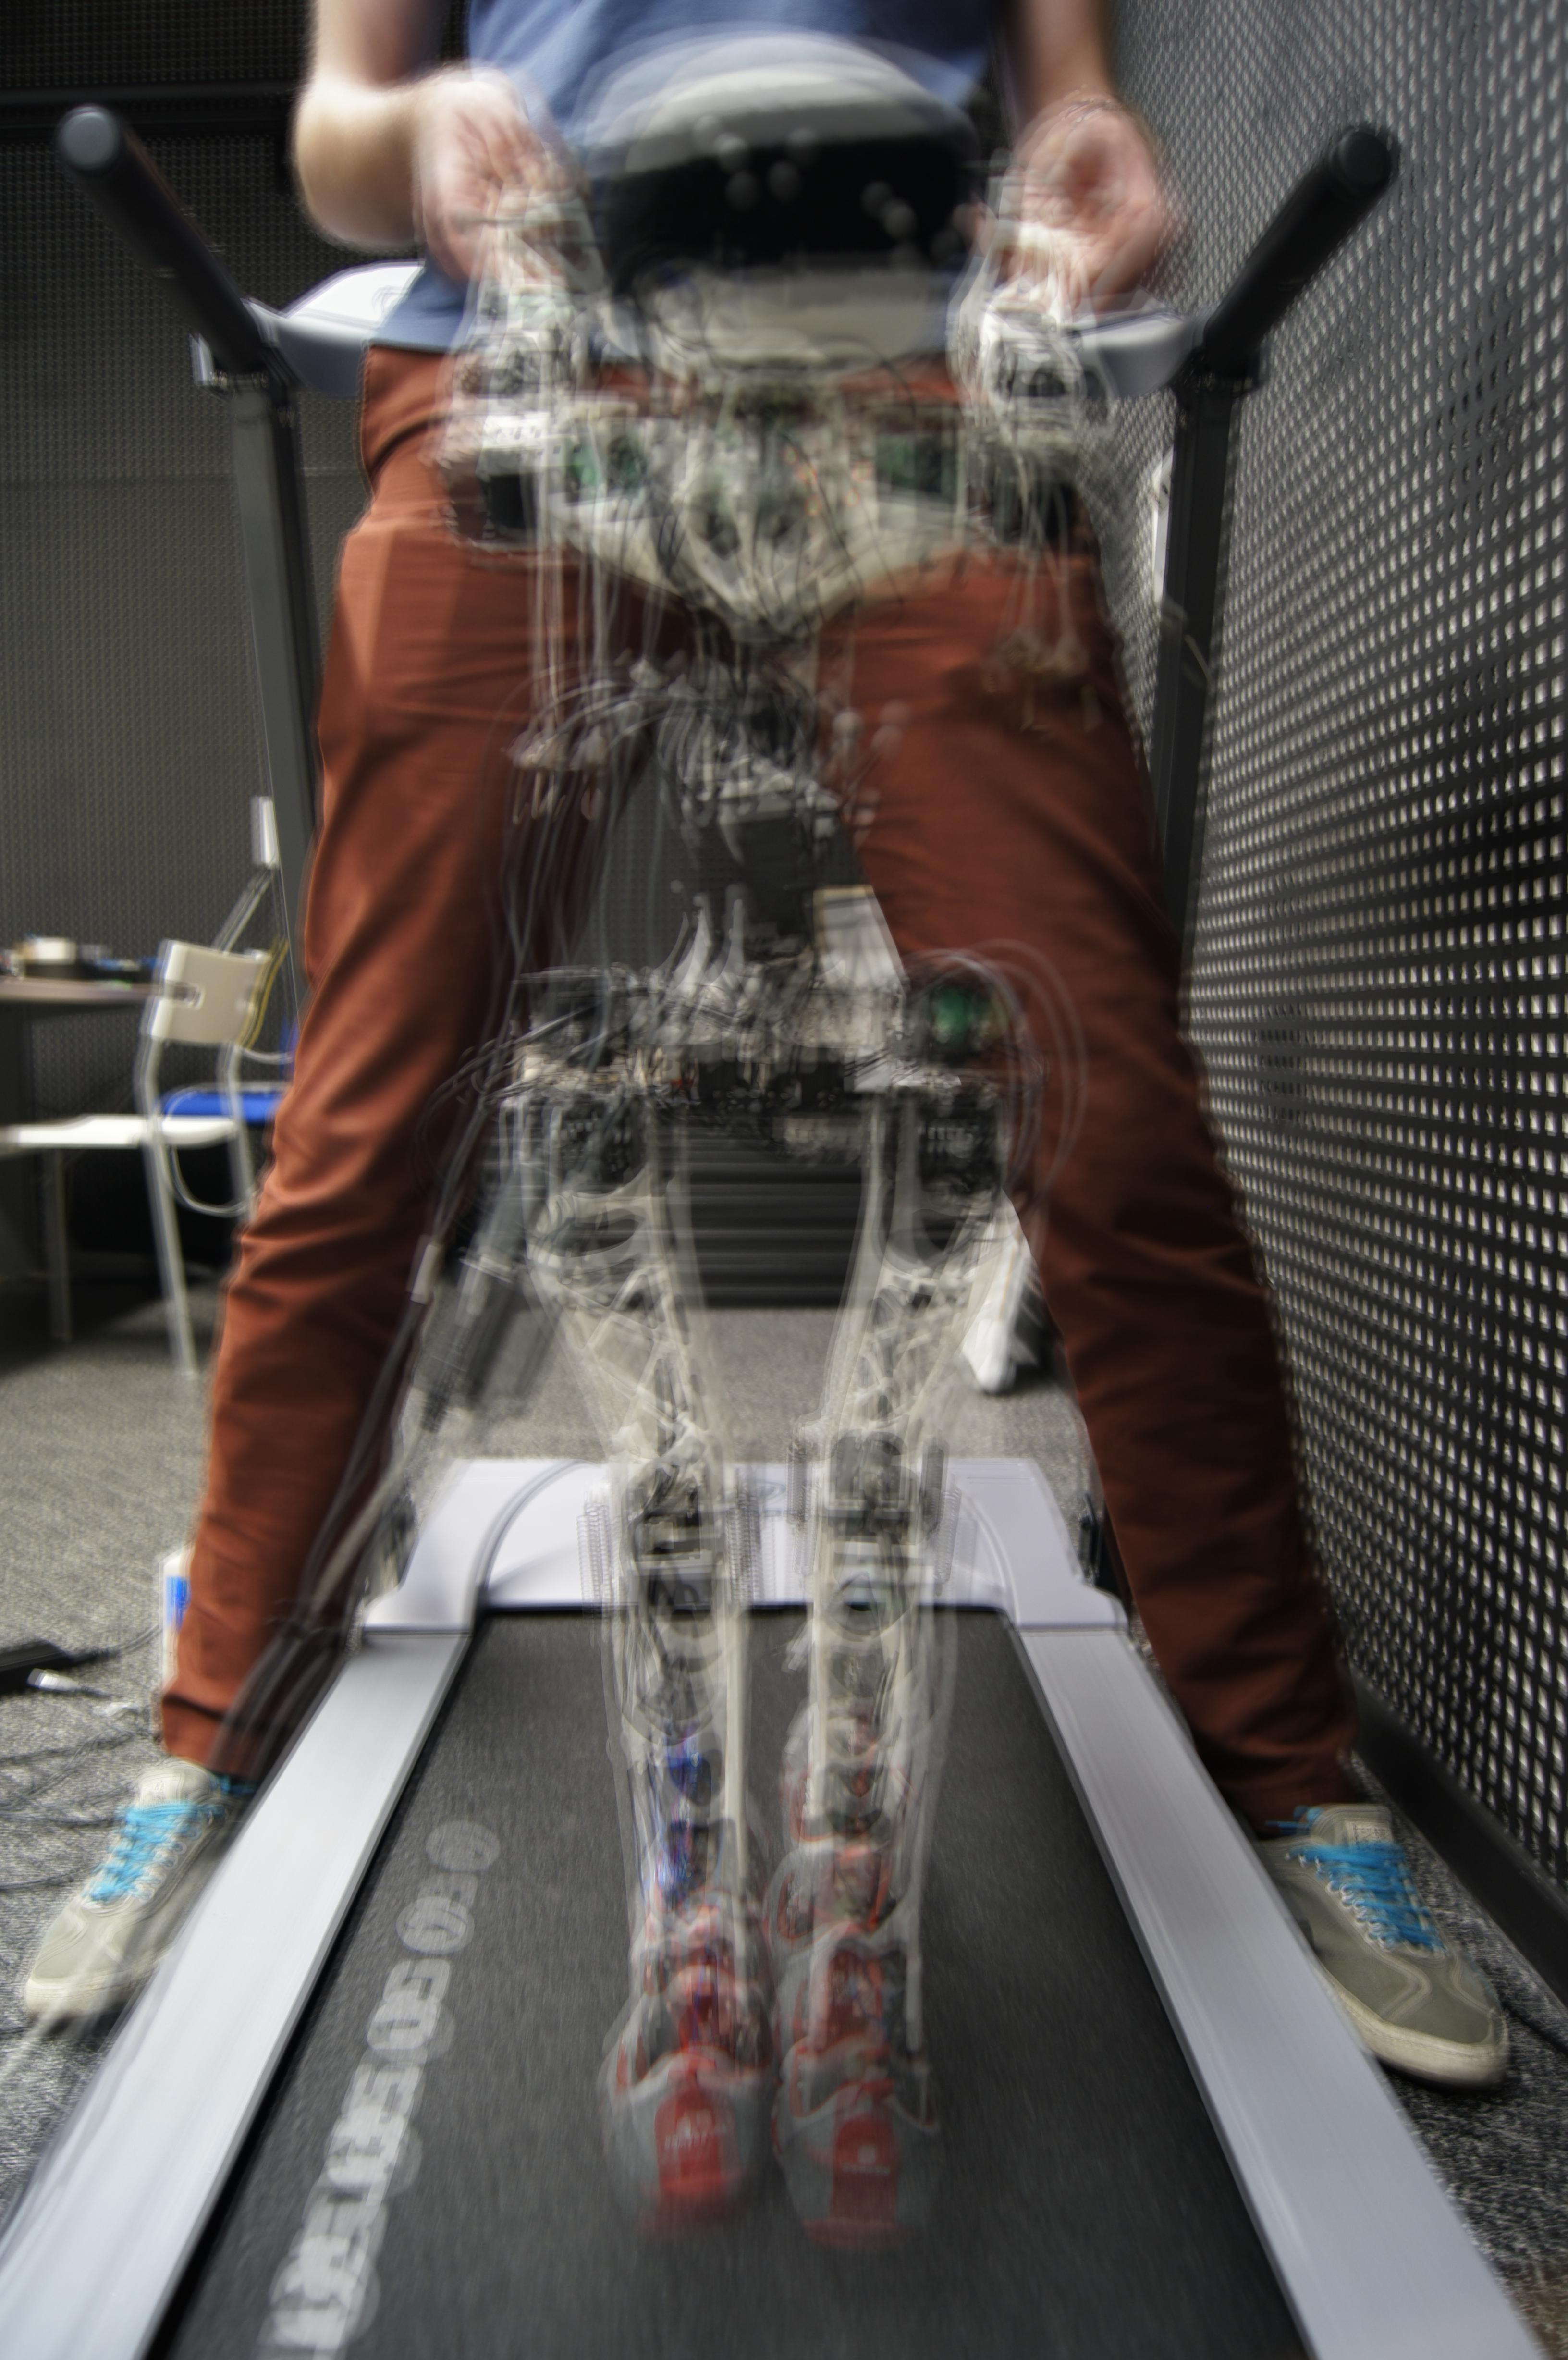
\includegraphics[width=0.49\linewidth]{marche_bended.jpg}}
    \hfil
    \subfloat[][straight thigh]{\label{fig:poppy_walking_straight}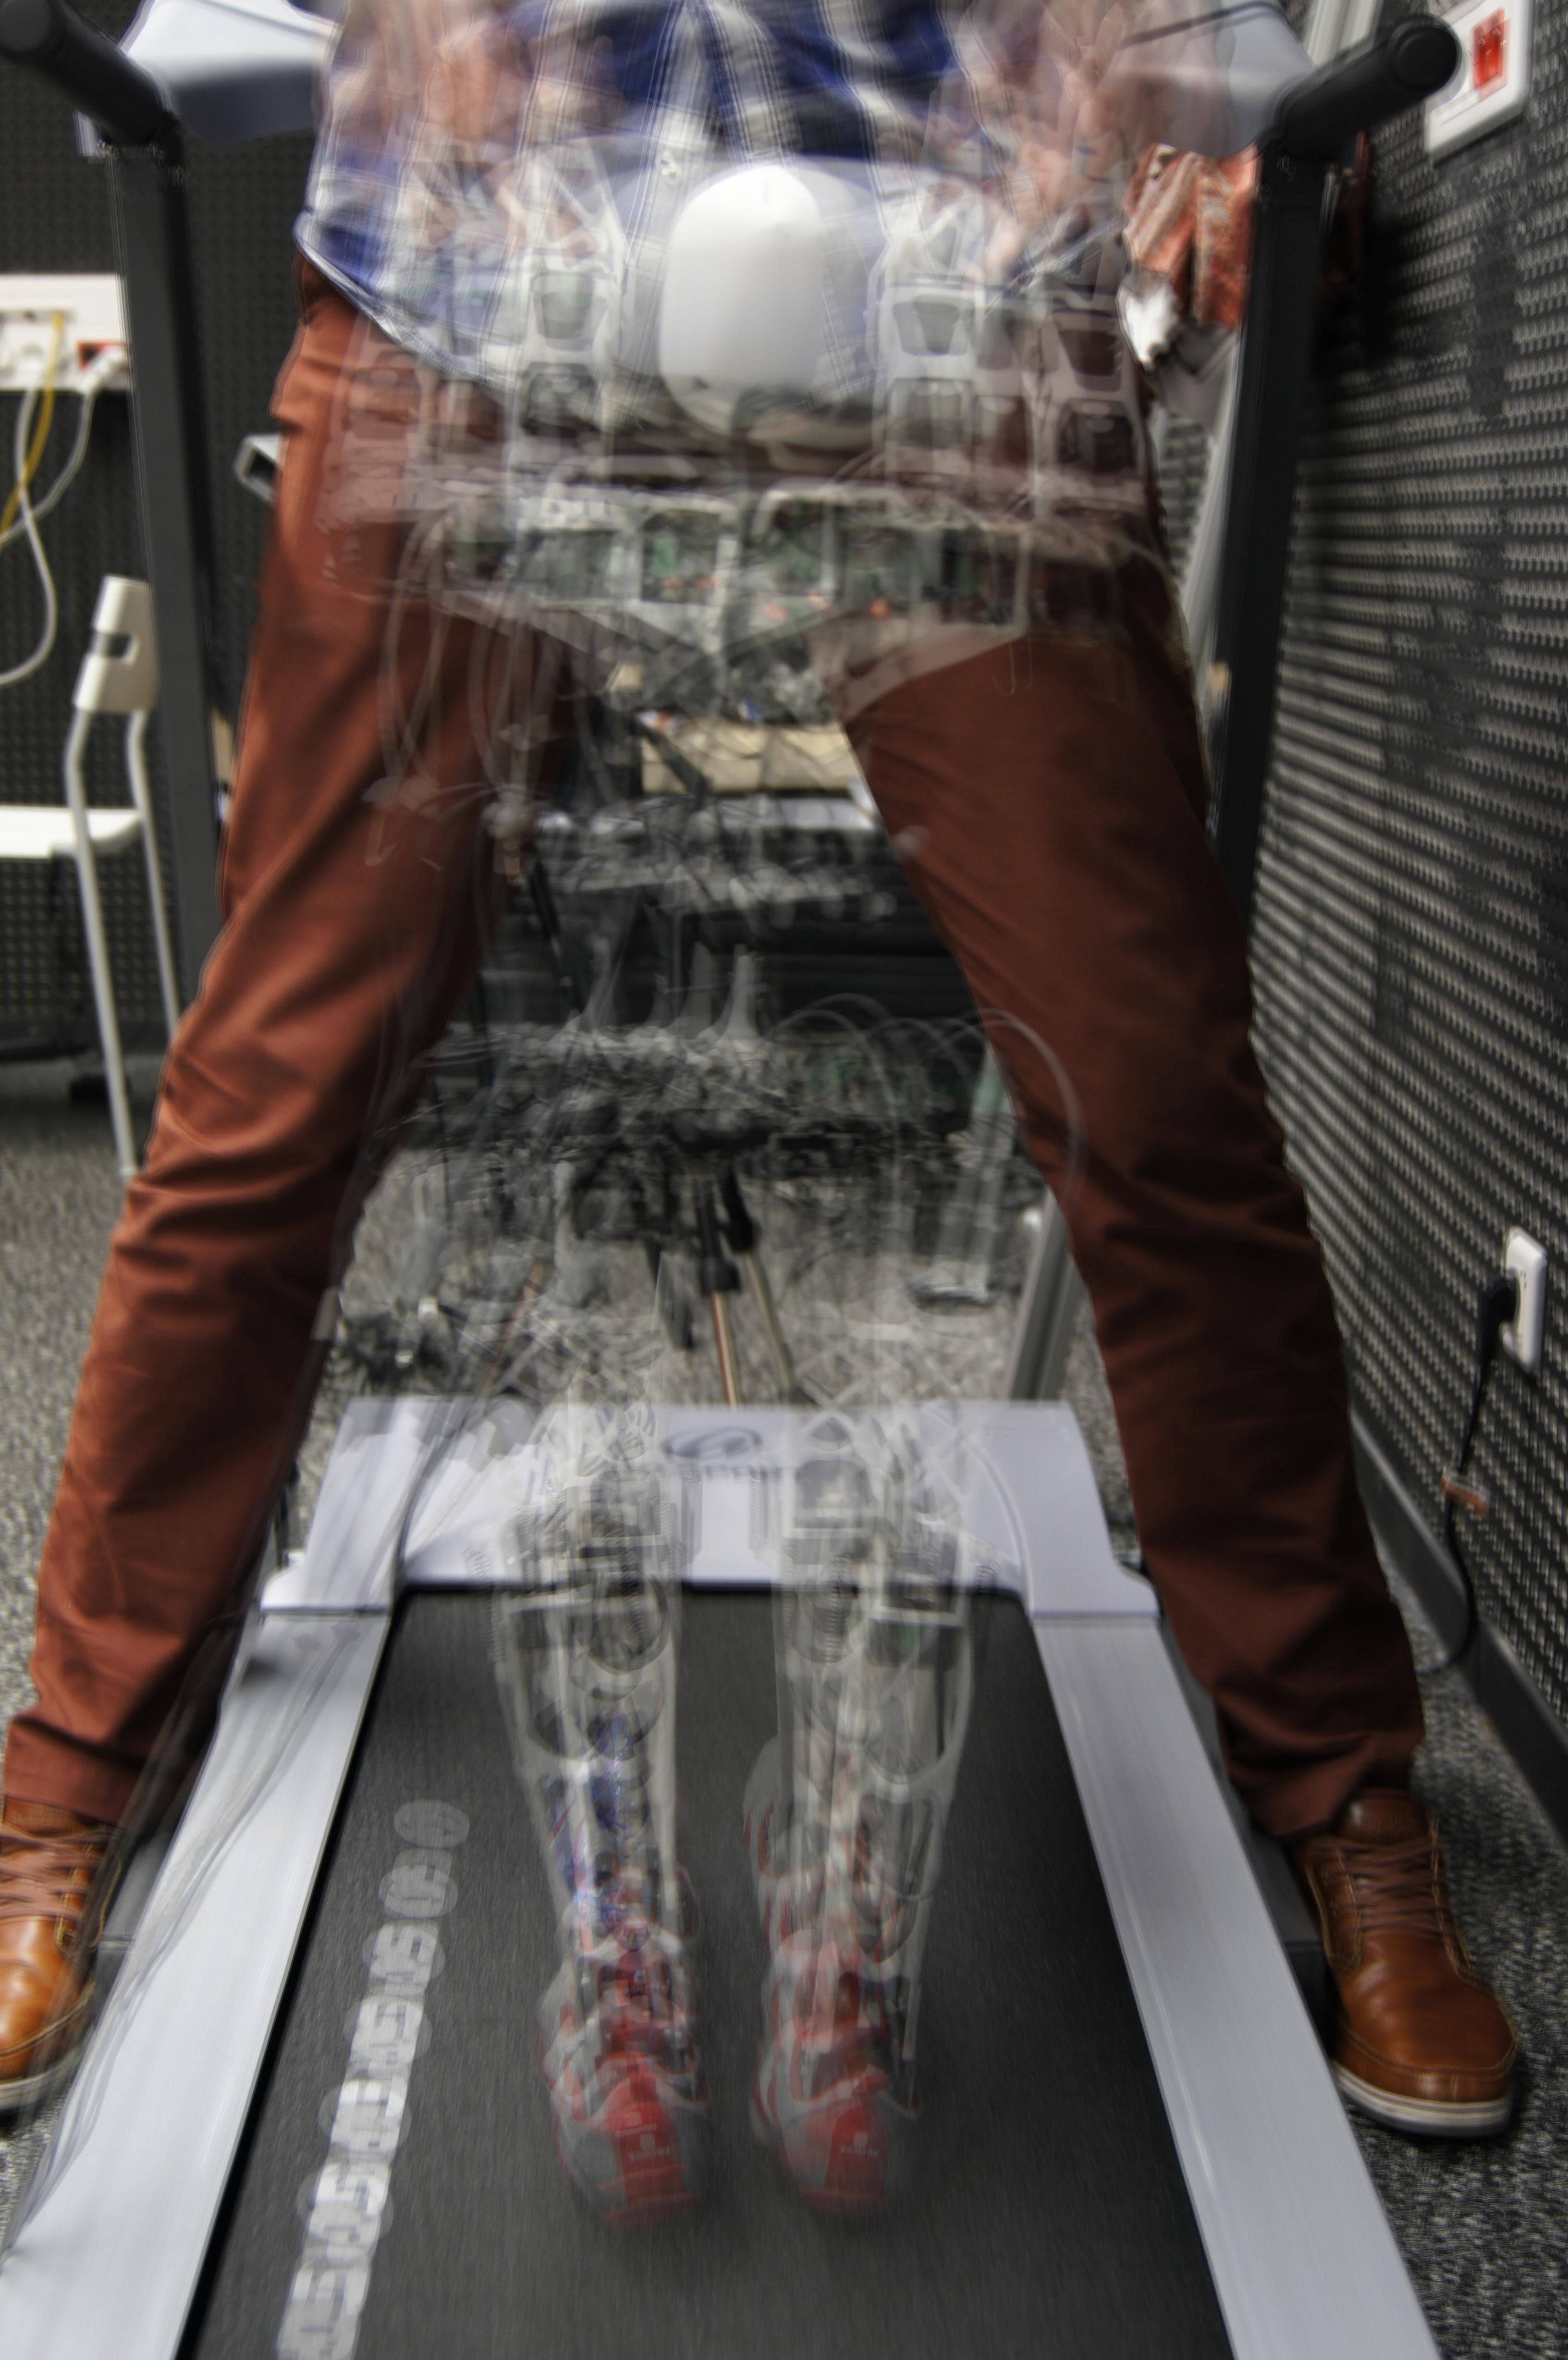
\includegraphics[width=0.49\linewidth]{marche_straight.jpg}}
    \caption{Five pictures have been taken while Poppy was walking and were stacked to obtain a qualitative view of the difference in the walking behavior in relation to the morphology of the thigh.}
    \label{fig:poppy_walking_compared}
\end{figure}


\subsection{Conclusion on the thigh shape role for bipedal locomotion} % (fold)
We focus on the shape of the Poppy thigh and its effect on the robot’s dynamic. We studied the role of morphology in the reduction and simplification of the control needed to perform complex task such as bipedal walking. We have presented the simple theoretical model we used for the design of Poppy’s thigh based on the inverse pendulum dynamic. We have conducted experiments to evaluate the improvements of the bended thigh on the real robot dynamic and compared it to the model. Since Poppy’s structural design allows easy, cheap and fast morphological modifications, we were able to try another thigh design. We also used a pair of straight thighs which is a more classical approach in humanoid conception. The experimental comparison between the two thighs design confirmed the theoretical results, the bio-inspired thigh design improves Poppy’s dynamic in two main ways useful for bipedal walking:
\begin{itemize}
    \item It reduces the falling velocity by almost 60\% when the robot is on one foot (single support phase).
    \item It reduces the lateral motion needed to transfer the mass of the robot from one foot to the other (double support phase) by 30\%.
\end{itemize}
It is really interesting to note that such a small modification of the robot morphology has a very significant impact on the robot’s behavior.

These results are interesting but they do not reflect the Poppy’s real walking dynamic. To evaluate the effect of the bended thigh on bipedal locomotion, we conducted a third experiment where Poppy is walking on a treadmill. In this experiment, we show that the bended thigh has an effect on a complex dynamic task such as the biped locomotion: it reduces the motion amplitude on the upper body  by 45\% and increases the head stability by 30\%. We choose these metrics due to our experimental constraints (fixed speed, social guidance) as a qualitative evaluation of the walking gait. Moreover it provides us with an intuitive, yet incomplete evaluation of the walking. Many other measures could have been chosen or combined such as speed, energy consumption or robustness to external perturbations. It is still complicated to understand which metric is the most adapted for robotic biped locomotion. As human beings are trained to recognize a bipedal gait, users can provide guidance to the robot for both safety of exploration and evaluation of the walking behavior.


% subsection Results (end)


% !TEX root = ../../thesis.tex

\newpage
\section{Rapid morphological exploration} % (fold)
\label{sec:morphology-variable}

In the previous section we showed how Poppy can be used to explore the actual role of morphology for humanoid behaviours. However, Poppy is a prototyping platform designed to test and experiment quickly several technological solution, especially thanks to modular properties, but until now, we did not actually evaluate it.

Therefore while we were working on a new design for Poppy's feet and exploring a design similar to "foot 1" (see \figurename~\ref{fig:pic_foot_1}), we decided to use this as a context to conduct an experiment into multiple variations of the foot morphology as an illustration of the methodology we have initiated with Poppy and presented in section REF.


The aim of this experiment is to quickly explore the effect of foot morphology on stability. Here, we are particularly interested in the stability of the head after a stepping impact. These impacts are quite challenging to simulate realistically and the natural compliance of the Poppy platform means it is even more important to test this on the real robot.

For the sake of lightness, the initial design of Poppy's feet only had one degree of freedom (DoF): pitch rotation. This configuration carried the inconvenience of preventing a proper parallel foot/ground contact. Thus, we developed several different feet with two degrees of freedom. Along with a standard motorized 2 DoF flat foot design, we also wanted to explore passive joints with springs. The use of passive joints allows for both lightness and reactive torque for stability.


\begin{figure}[p]
\centering
    \subfloat[][Foot\_1]{\label{fig:pic_foot_1}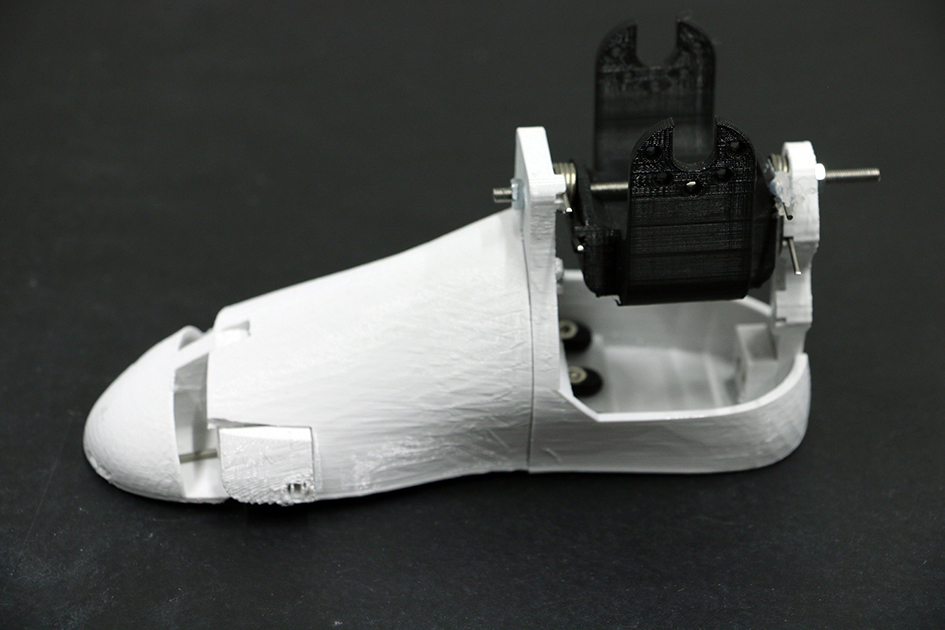
\includegraphics[width=0.45\linewidth]{pic_foot_1.JPG}}
    \hfil
    \subfloat[][Foot\_2]{\label{fig:pic_foot_2}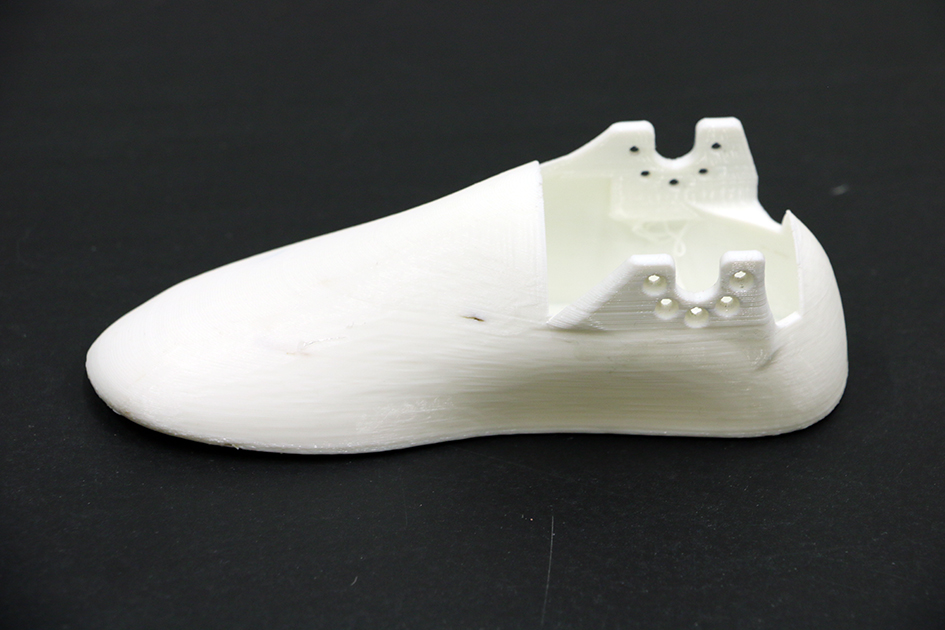
\includegraphics[width=0.45\linewidth]{pic_foot_2.JPG}}\\
    \subfloat[][Foot\_3]{\label{fig:pic_foot_3}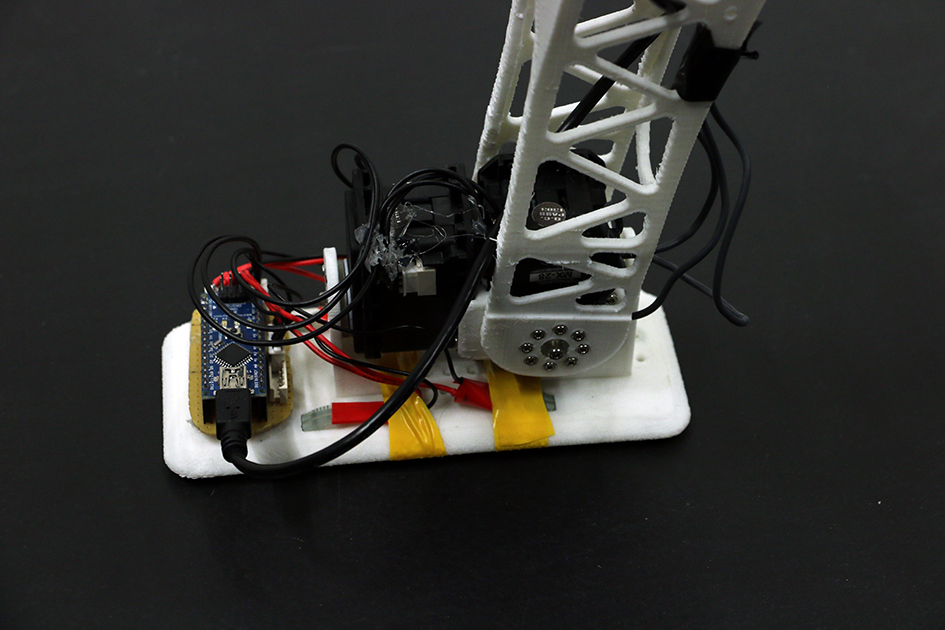
\includegraphics[width=0.45\linewidth]{pic_foot_3.JPG}}
    \hfil
    \subfloat[][Foot\_4]{\label{fig:pic_foot_4}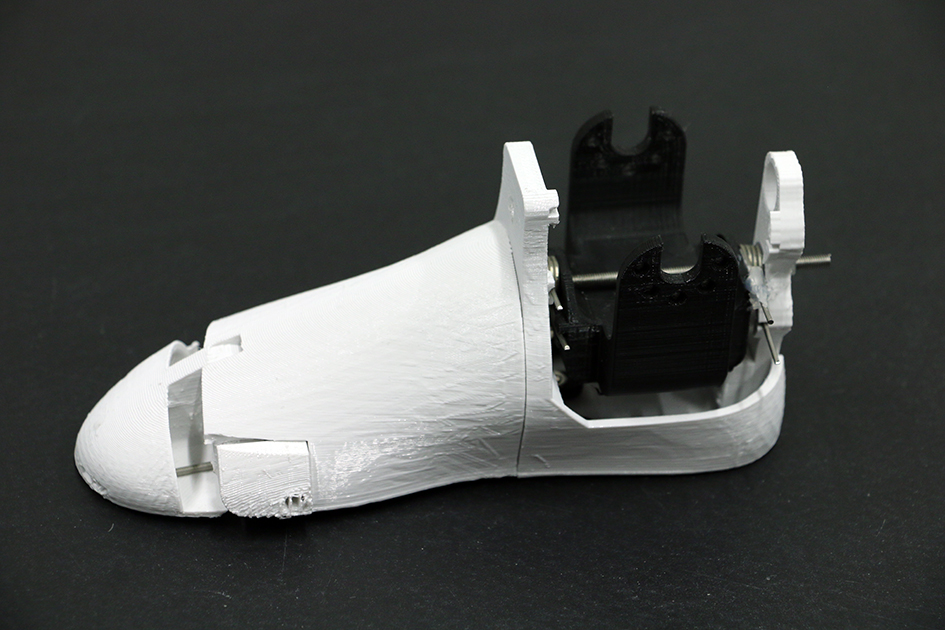
\includegraphics[width=0.45\linewidth]{pic_foot_4.JPG}}


    \subfloat[][Foot\_4]{\label{fig:foot_experience_blueprint}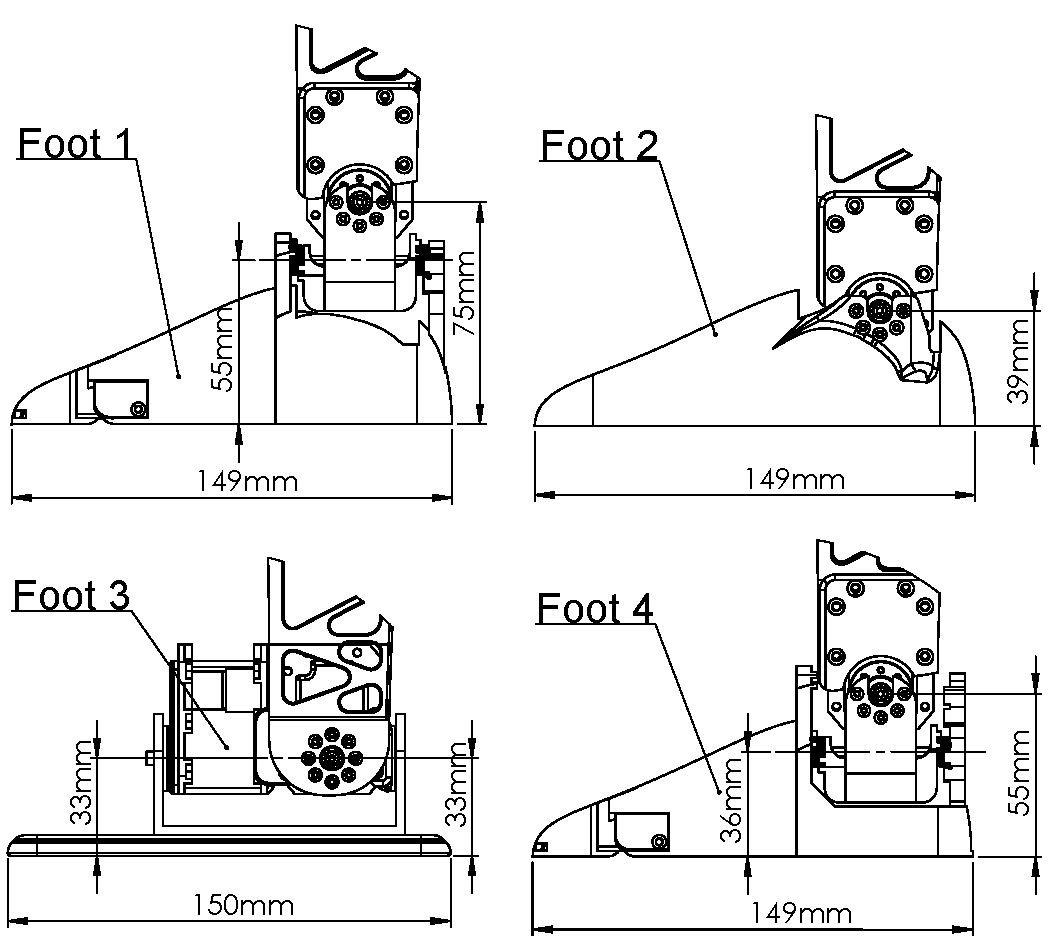
\includegraphics[width=0.95\linewidth]{foot_experience.pdf}}
    % \subfloat[][]{\label{fig:pic_shoe}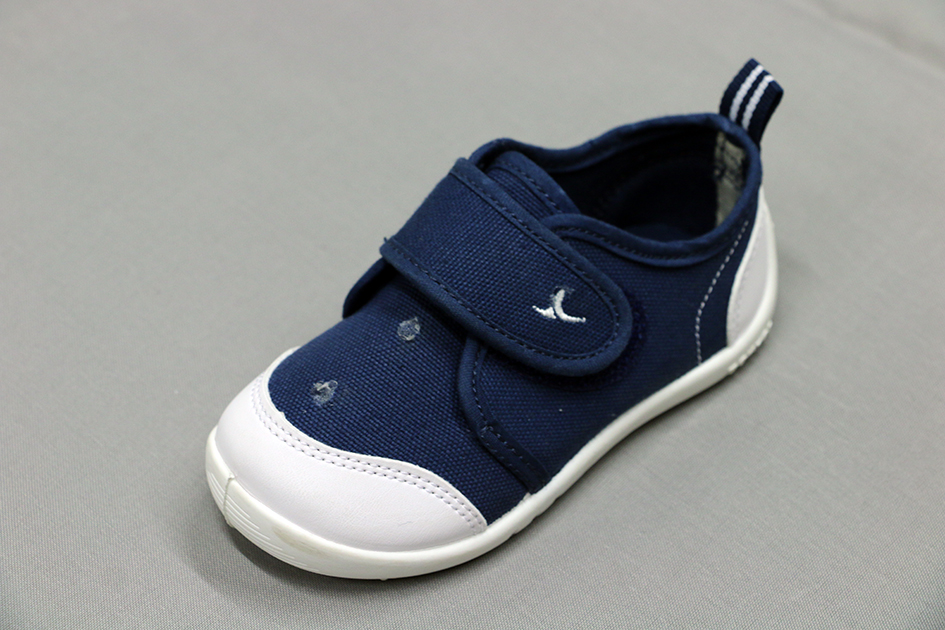
\includegraphics[width=0.48\linewidth]{pic_shoe.JPG}}
    \caption{}
    \label{fig:foot_variants}
\end{figure}


\begin{table}
    \begin{center}
        \begin{tabular}{|l|c|c|c|c|}
        \hline
        \textbf{Type} & \textbf{Foot 1} & \textbf{Foot 2} & \textbf{Foot 3} & \textbf{Foot 4}\\
        \hline
        \textbf{Double rotation} & Passive & No & Active & Passive\\
        \hline
        \textbf{Human-like foot} & Yes & Yes & No & Yes\\
        \hline
        \textbf{Toes} & Yes & No & No & Yes\\
        \hline
        \textbf{Rotation axis height} & 75.70 mm & 33 mm & 39 mm & 35.5 mm\\
        \hline

        \end{tabular}
        \caption{Table summarizing the different types of feet used.\\
        \textbf{Passive double-rotation:}  one active rotation (motor: Dynamixel MX 28) for the sagittal plan and a passive rotation for the frontal plan with two springs.\\
        \textbf{Active double-rotation:}  A two motorized rotations (sagittal plan and frontal plan). No double-rotation:  one motorized rotation (sagittal plan).\\
        \textbf{Human-like foot:} a foot design resembling a human foot of a two year-old child (size: 130.7 mm shoes size: 23 EU). The feet were tested with and without shoes.\\
        \textbf{Rotation axis height:} the height between the axis of rotation of the sagittal plan and the floor without shoes.\\
        \textbf{Toes:} Indicates that the foot has toes.
        }
        \label{tab:table_feet}
    \end{center}
\end{table}


Moreover, it appeared that a proper foot/ground contact with convenient friction was difficult to obtain based only on 3D-printed material. One simple solution to this problem is to use a shoe which can provide a high friction and adapt slightly to imperfections on the ground. Furthermore, this solution also allows keeping the feet close to humans ones. Thus, the feet tested (with the exception of the flat foot) were designed from a moulding of the interior of a shoe. It is to be noted that we also included passive toes (with springs) on some of the feet tested for future work on locomotion. These toes should not have any significant impact on the criterion tested.


\subsection{Experimental setup} % (fold)
\label{sub:experimental_setup}

For this experiment, the robot simply stands upright secured by a slack strap on a fixed gantry. Different markers on the robot are tracked by a motion capture system at 100Hz (Natural Point OptiTrack). See figure \ref{fig:setup} for more details.

\begin{figure}[ht]
    \begin{center}
        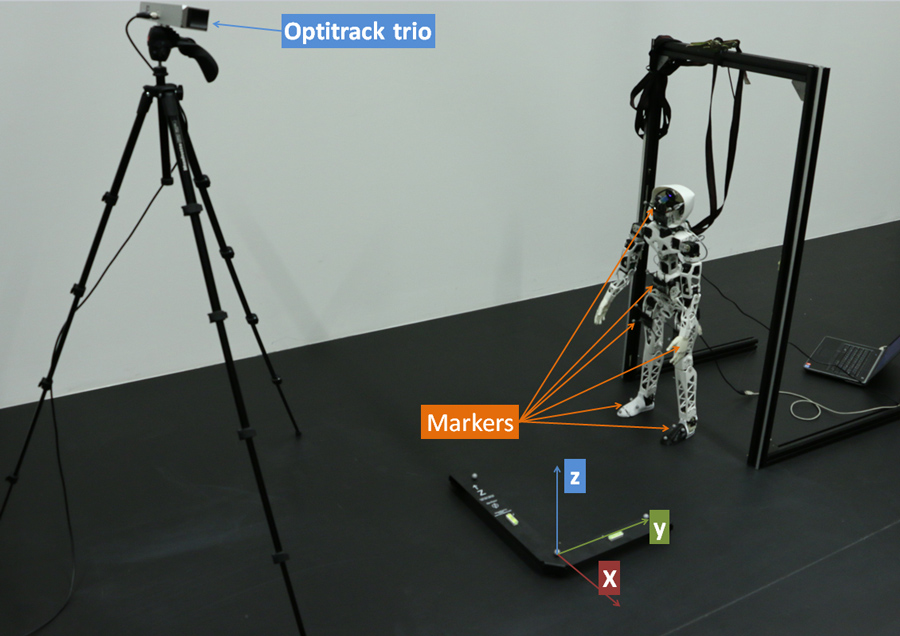
\includegraphics[width=0.9\linewidth]{pic_setup.jpg}
    \end{center}
    \caption{Experimental setup. The robot is secured by slack strap on a gantry and tracked by an OptiTrack trio device. Markers are placed on the feet, hips, abdomen, and on the head}
    \label{fig:setup}
\end{figure}

Four different feet were tested (cf. Table~\ref{tab:table_feet}). Three out of the four feet were tested both with and without shoes.


\subsection{Experiments} % (fold)

The feet were tested with a very simple discrete movement (see \codename~\ref{code:foot_mouvement}), representative of the kind of impacts that occur during walking. The robot performs a single step leftward with the left leg. The left foot is lifted (3cm) and then put back on the ground with a slight lateral displacement towards the exterior (5° at the level of the hip). The duration  of the whole movement is about 0.4 s and repeated 20 times for each configuration.

\lstinputlisting[
    language = Python,
    caption = {Discrete mouvement executed on Poppy},
    label = {code:foot_mouvement},
    float = p]
    {code/foot_mouvement.py}


\subsection{Results} % (fold)

Figures \ref{fig:head_x}, \ref{fig:head_y} and \ref{fig:head_z} respectively show the evolution of the position of the head marker in the $x$, $y$ and $z$ axis for each foot tested. Dotted vertical lines indicate the beginning and the end of the leg movement.

These figures show that the dynamics of the robot are not trivial, even for the simple movement we tested, the standard deviation is not negligible and shows how chaotic the reaction of such an impact can be. This particularity is another proof of the significance of the use of experimentation versus simulation.

We can clearly see that foot 3 (standard flat foot) behaves quite differently than the other feet tested. In particular in the $x$ and $y$ directions, we see that with this foot the head tends to move more towards the exterior (left of the robot) and towards the rear.
%% These differences may be explained by the larger ground contact surface
%% provided by the flat feet.

Regarding the effect of the shoes, results are less clear but most of the time (except for foot 1) differences occur between a given foot with and without shoes. The friction with the ground can explain these differences. Bare feet tend to slip more than those with shoes.


\begin{figure}[ht]
    \begin{center}
        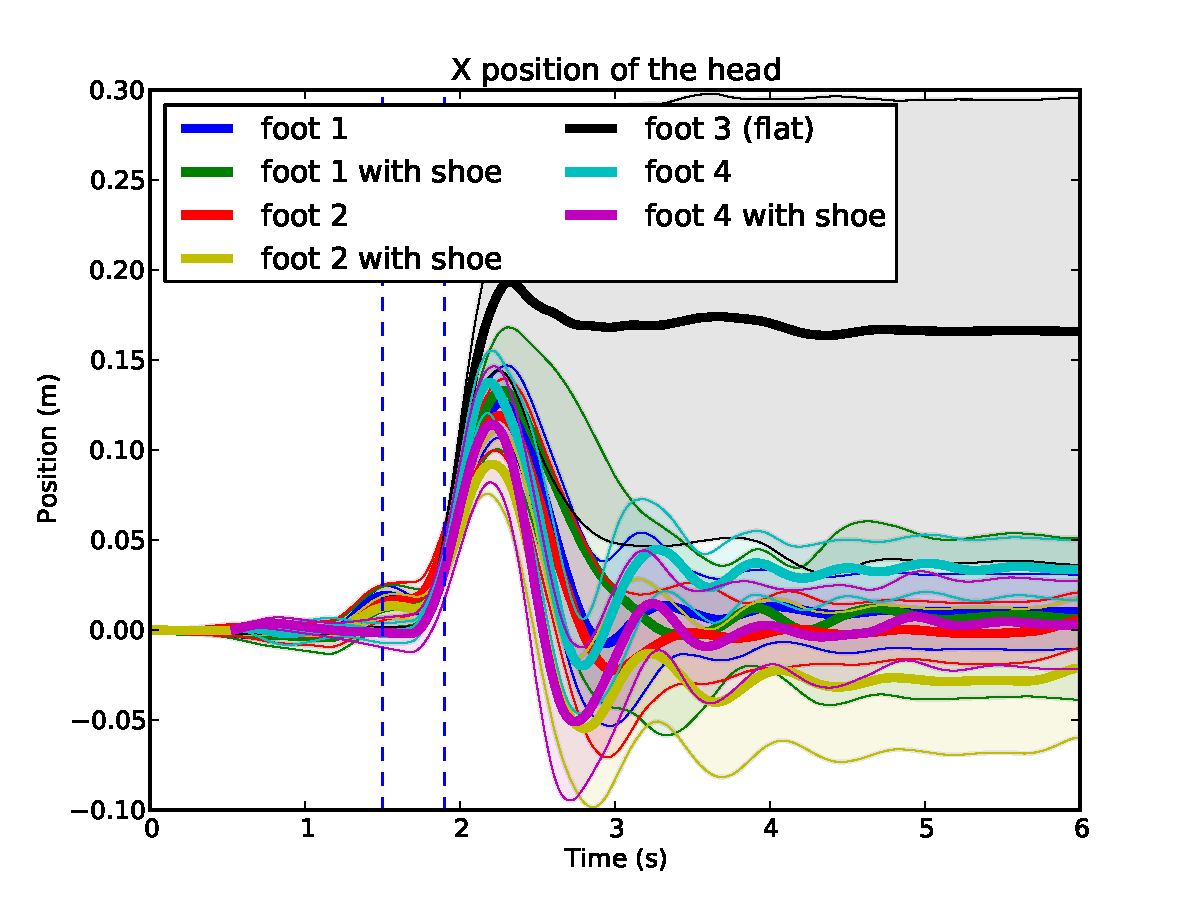
\includegraphics[width=\linewidth]{head_x.pdf}
    \end{center}
    \caption{Evolution of the position of the head in the $x$ axis for
    each foot tested (see \figurename~\ref{fig:foot_variants} for illustration of each foot)}
    \label{fig:head_x}
\end{figure}

\begin{figure}[ht]
    \begin{center}
        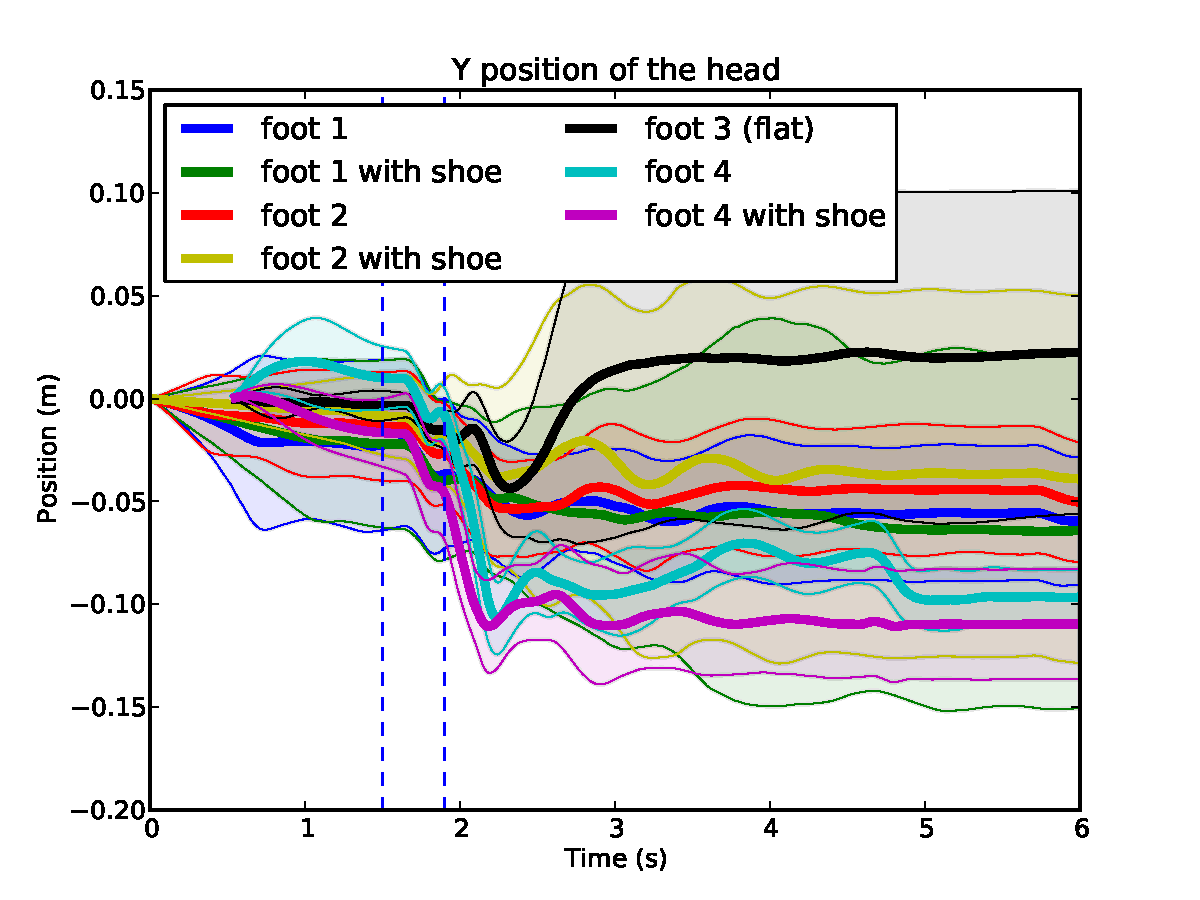
\includegraphics[width=\linewidth]{head_y.pdf}
    \end{center}
    \caption{Evolution of the position of the head in the $y$ axis for
    each foot tested (see \figurename~\ref{fig:foot_variants} for illustration of each foot).}
    \label{fig:head_y}
\end{figure}

\begin{figure}[ht]
    \begin{center}
        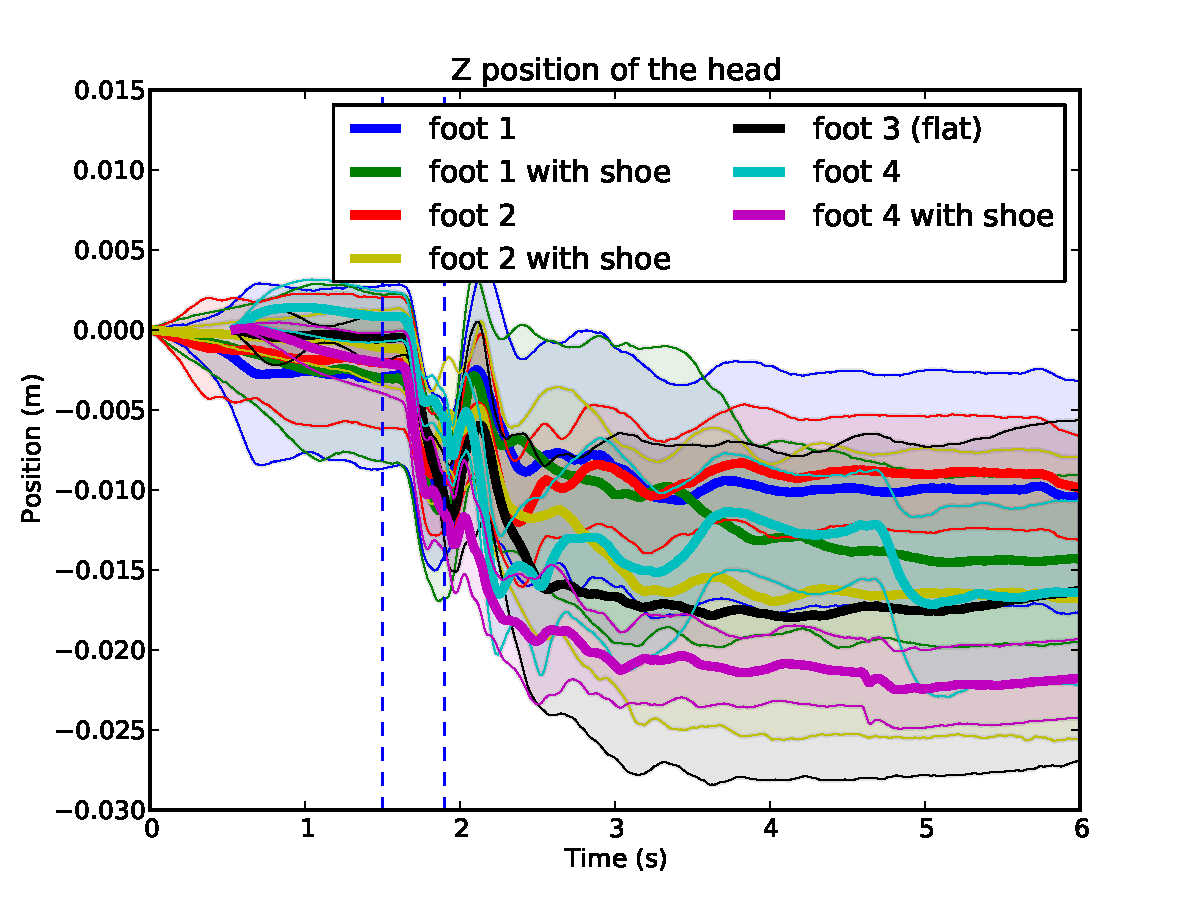
\includegraphics[width=\linewidth]{head_z.pdf}
    \end{center}
    \caption{Evolution of the position of the head in the $z$ axis for
    each foot tested (see \figurename~\ref{fig:foot_variants} for illustration of each foot).}
    \label{fig:head_z}
\end{figure}


This first experiment allowed us to determine that the use of an active double rotation of the ankle may not be mandatory. Indeed, the behaviors observed with the passive feet were even better than with the flat feet with active rotation. Although a clear interpretation of this phenomenon is still difficult to propose, some hypotheses related to the weight (with one more motor feet are heavier) and the area of surface in contact with the ground (flat foot surface is bigger) have to be investigated.

Moreover, we observed that the shoes added extra friction in relation to the ground without really impairing the stability. Although rarely used in humanoid robotics, these early results encourage us to explore this possibility in more depth.

Finally the most important aspect for us was to actually evaluate the amount of time needed to conduct such experiments with Poppy. The starting point was "foot 1" as it was the work in progress. Thus morphological design modifications only concern foot 3 and 4:
\begin{itemize}
    \item \textbf{Foot 3 (flat):} Modifying Poppy’s initial foot design to permit the integration of two Dynamixel motors and the associated flat feet required 16 hours of CAD design. The printing of the whole required part (2 legs, 2 feet and 2 ankles) took approximately 30 hours on a low-cost FDM printer (Makerbot Replicator 2).
    \item \textbf{Foot 4:} While the difference with foot 1 concerns only one parameter (i.e. the joint position), the modification needed to produce foot 4 based on foot 1 was done in approximately 2 hours of CAD. Then the printing of the new part was achieved in 10 hours.
\end{itemize}

Then, conducting the whole experiment (i.e. design the leg motion, establishment of the experimental setup and data acquisition) was achieved in about one week with two people. \textbf{In particular, the actual experimentation involving changing Poppy's feet seven times and acquiring at least 20 trials for each took less than two days.}

\subsection{Reuse of this experiment} % (fold)

Everything necessary to obtain and use Poppy is available on our GitHub project page: \url{www.github.com/poppy_project}. Also, to complete the illustration of this Poppy use-case, we diffuse along with the present paper:
\begin{itemize}
     \item the whole setup materials i.e. the code used for the experiment and the 3D files to reproduce/modify each foot,
     \item the raw data acquired that include for each trial: all markers position, head IMU measurement and the complete motors data (proprioceptive position evaluation overtime),
     \item the code used to extract and plot the results presented.
\end{itemize}

All these materials are available on the repository associated with this experiment: \url{https://github.com/matthieu-lapeyre/Humanoids2014} and can be freely used e.g. for further investigation with the acquired data, or to reproduce and extend the experiment.


% !TEX root = ../../thesis.tex
\newpage
\section{Adding novel mechanisms to Poppy} % (fold)
\label{sec:morphology-add-mechanism}

\textbf{context:} Poppy has been made to allow quick and cheap exploration and experimentation of morphological variation (i.e. change of its hardware).
\textbf{need:}
We are interested in the design of increasingly under-actuated robots. We especially want to explore semi-passive ability and use of natural body properties rather than using actuation power to achieve dynamic tasks. Until now,  humanoid bipedal locomotion has mostly been achieved using ZMP control leading to walking gait with the knees always bended. The permanent high torque and foot impacts applied to the knee require high-powered actuators.
\textbf{Task:} With Poppy, we wanted to explore a mechanical design that reduces the required power. We decided to test the use of a semi-passive knee joint based on a MX-28 Dynamixel motor completed with a parallel spring system.
\textbf{objet:} We will explain how we create this mechanism by changing the mechanical design of Poppy's legs and we will present the results we obtained during walking experiments.

We explore the design of a semi-passive mechanism with the aim of assisting the motor during two critical phases of the walking gait:
\begin{enumerate}
    \item the foot impact, which can produce an abrupt raise of load in the knee during stance phase,
    \item the flexion of the leg during swing phase.
\end{enumerate}

\subsection{Semi-passive knee mechanism principle} % (fold)
For this purpose we chose a mechanism inspired by that of Gini and Scarfogliero~\cite{gini2009new} involving two traction springs positioned in parallel to the knee joint in such a way that there are two low-potential solutions, one when the leg is straight and one when the leg is bended (see \figurename~\ref{fig:Gini_knee}).

\begin{figure}[]
\centering
    \subfloat[][Actual design of the robot knee.]{\label{fig:}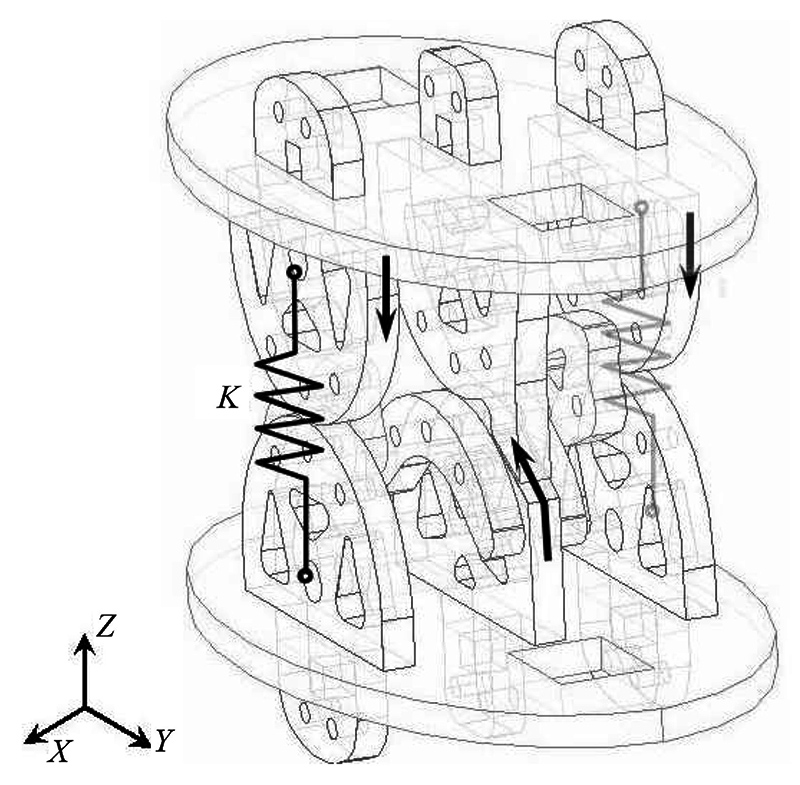
\includegraphics[height=5cm]{Gini_knee_design.jpg}}
    \hfil
    \subfloat[][Mechanism principle.]{\label{fig:}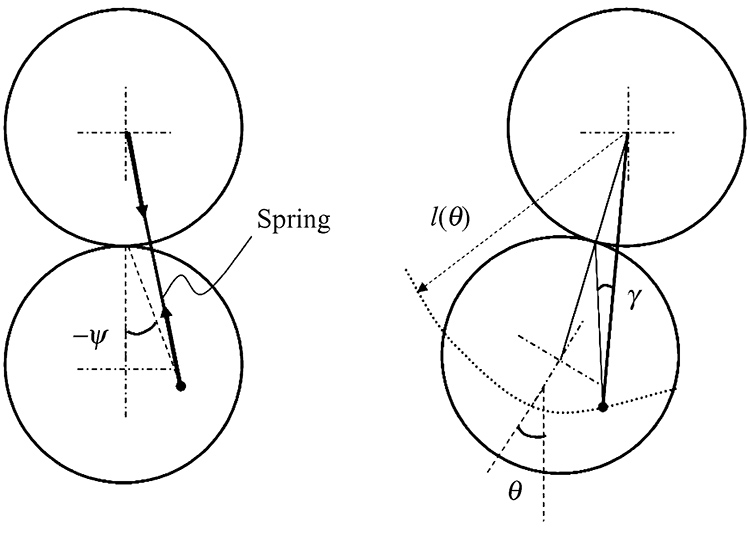
\includegraphics[height=5cm]{Gini_knee_mechanism.jpg}}
    \caption{Gini and Scarfogliero designed a bio-inspired knee joint which uses parallel traction springs to both bend the leg and keep it straight. Illustrations extracted from~\cite{gini2009new}.}
    \label{fig:Gini_knee}
\end{figure}

Therefore this mechanism can participate in the leg dynamic and assist the motor during two walking main phases:
\begin{itemize}
    \item They help to keep the leg straight during the support phase without any motor control.
    \item During the swing phase, they participate in the flexion of the leg.
\end{itemize}

These two modes can be passively switched by the actual knee angle, yet we have to determine which angle is the most suitable. Considering the human knee kinematic (see Fig.~\ref{fig:human_knee_kinematic}), we chose to change mode at $\theta_{knee} = 20+5$\textsuperscript{o}  which corresponds to a transition between the stance preparation phase and the swing phase.

\begin{figure}[thpb]
    \centering
    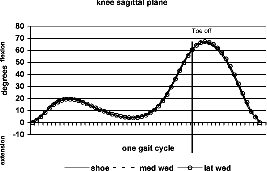
\includegraphics[width=0.6\linewidth]{knee_kinematic.pdf}
    \caption{Actual flexion kinematic of a human knee during the walking gait~\cite{Nester2003}. We can identify two main phases corresponding to the stance preparation phase and the swing phase. The main difference is the amplitude of the motion i.e $<20$\textsuperscript{o}  for the stance phase and $>20$\textsuperscript{o} for the swing phase.}
    \label{fig:human_knee_kinematic}
\end{figure}


\subsection{Experimentation on Poppy} % (fold)

An illustration of the real behavior is shown in the videos \url{https://vimeo.com/63839782}

\begin{figure}[h]
    \begin{center}
        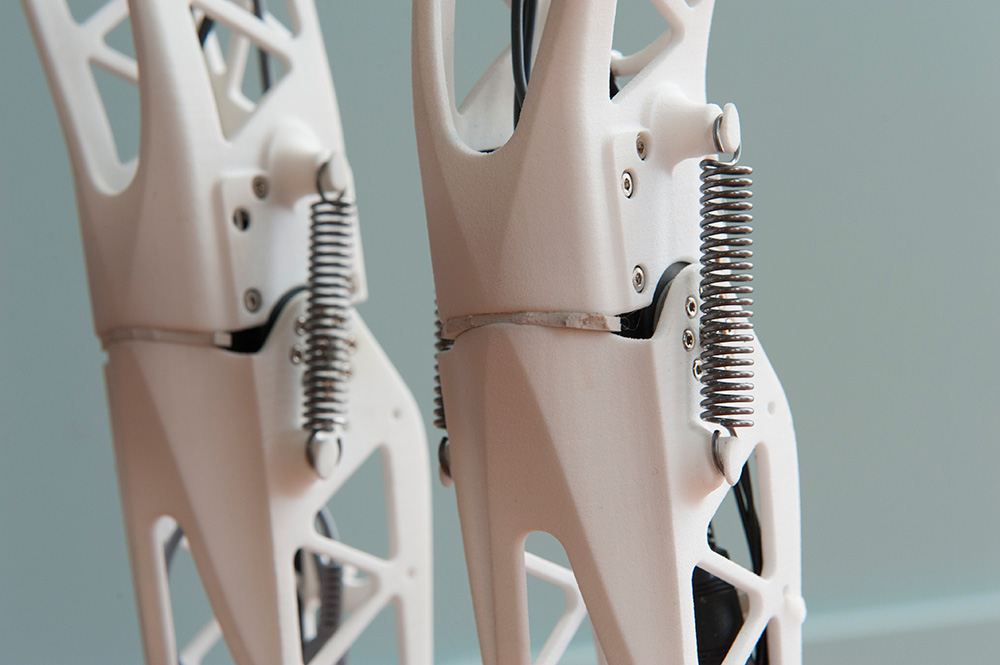
\includegraphics[width=0.6\linewidth]{poppy_semi_passive_knee.jpg}
    \end{center}
    \caption{Caption here}
    \label{fig:figure1}
\end{figure}


\begin{figure}[!h]
\centering
    \subfloat[][without springs]{\label{fig:knee_wout_spring}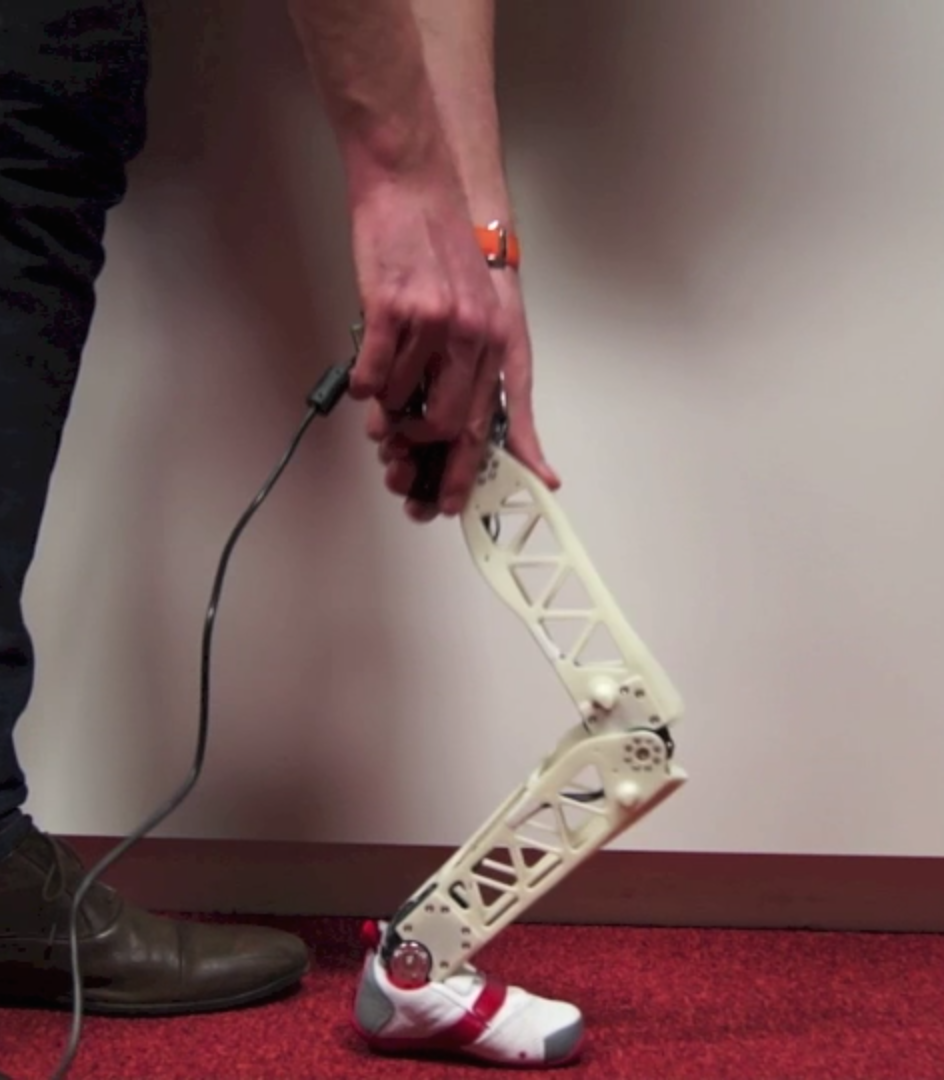
\includegraphics[height=6cm]{knee_wout_spring.png}}
    \hfil
    \subfloat[][with traction spring]{\label{fig:knee_w_spring}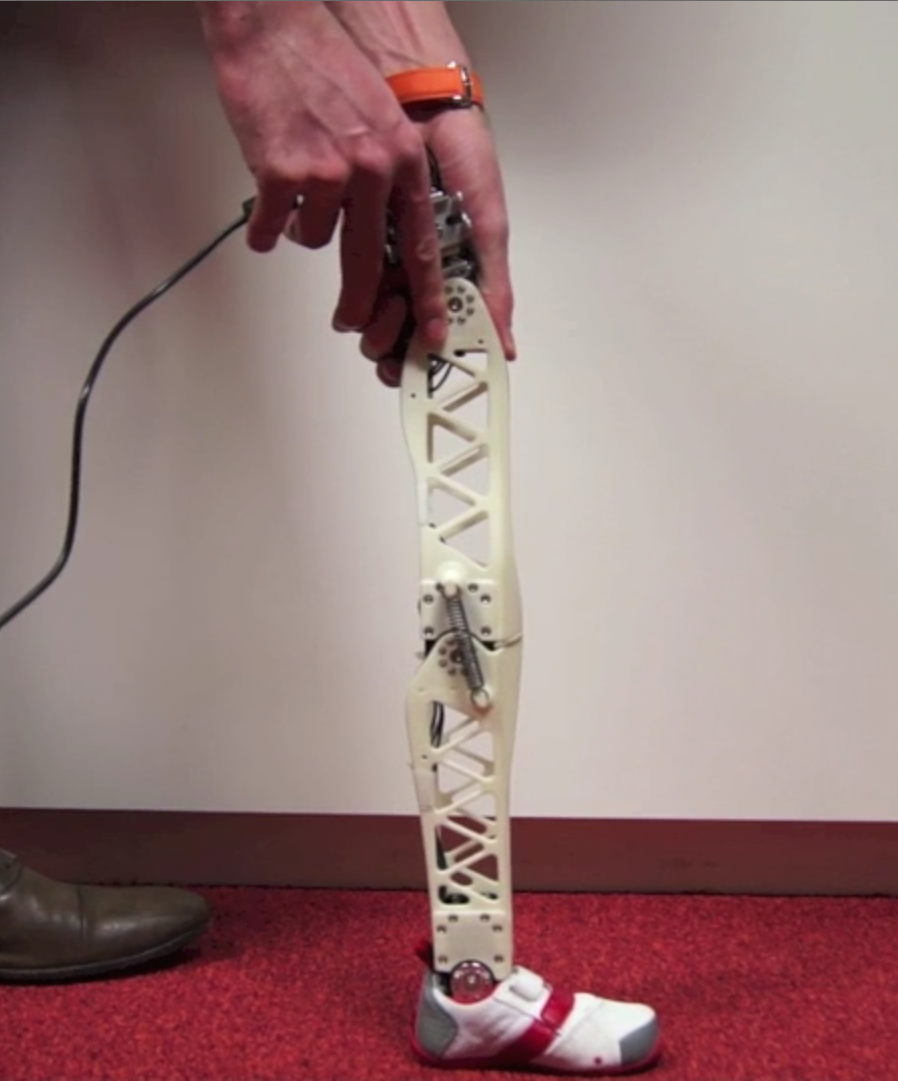
\includegraphics[height=6cm]{knee_w_spring}}
    \caption{Motors fully compliant \url{https://vimeo.com/63839782}}
    \label{fig:}
\end{figure}





% !TEX root = ../../thesis.tex

\newpage
\section{Extending the sensor apparatus of Poppy} % (fold)
\label{sec:morphology-adding-sensors}

Poppy has been designed following a methodology (presented in section~\ref{REF}) which makes easy the hacking of the platform.
The last experiments presented mechanical modifications of Poppy's morphology. Indeed thanks to its 3D printed structure, it is quite easy and straightforward to modify its mechanical parts, unfortunately we cannot (yet) print complex electronics circuits and components.

We therefore chose design a custom I/O board based on Arduino (detailed in section~\ref{REF}). As its name suggests, this board has for main purpose to ensure the several inputs/outputs of the robot and offers:
\begin{itemize}
    \item 2 Dynamixel buses (TTL),
    \item 2 internal USB and 2 external USB ports,
    \item analog and digital pins available on a classic Arduino Due which can be use as direct input/output or for communication buses such as UART, I2C or SPI.
\end{itemize}
Thus there are many more I/Os than required for Poppy. These extra ports has been intended to let Poppy users extend its sensorimotor space and adapt it to their needs.


During our first trials to design walking a primitive with Poppy, we have been interested in the measurement of under feet pressures but the simple foot design Poppy had, does not involve such sensors. With a traditional robotic platform, we should have to either use the available sensors, here the load measurement in the ankle Dynamixel motor, or add an external device with its own power supply and communication system.

With the Poppy electronic modularity, we can hack the robot and integrate new sensors. Then they can be plugged on the I/O board for communication and power supply needs.

To provide an example of how we can actually hack the Poppy robot, we will explain here what we did to integrate force sensors under the feet and acquire the data with the pypot library.


\subsection{Integration of foot pressure sensors on Poppy} % (fold)

To obtain measurement of the pressure variation under our Poppy's feet we used FSR sensors from Interlink Electronics (see \figurename~\ref{fig:FSR_explode_view}). The FSR sensor will vary its resistance depending on how much pressure is being applied to the sensing area. The harder the force, the lower the resistance is. The acquisition of the FSR value require to create a simple voltage-divider those the design is explained in appendix \ref{appendix:design_FSR}. These sensors are low-cost -6\$ each- yet theirs behaviors are very non-linear (see \figurename~\ref{fig:foot_sensor_behavior}) and the calibration is quite variable depending on the production batch and the thermal conditions. So we cannot expect having precise results.

When we did the integration of foot sensors on the Poppy, its feet were still a really simple and flexible 3D printed part. The actual force transmission was done by the shoes. We therefore had to directly attach the sensors below the shoes.
To avoid multiple wires (2 per sensor) going from the head to the feet, we decided to use additional arduino nano boards to acquire sensors values of each foot and stream the data through serial communication up to the IO board.

Because Arduino nano board has 8 analog inputs, we have added 8 sensors under each foot (see \figurename~\ref{fig:poppy_foot_sensors}) but actually only used 5 (the big ones) and integrated the arduino nano in the leg. While it was a hack of a real shoe and not just a print of new part, the intervention was quite annoying but still achievable in one day. Here we have chosen to use USB cable to plug each Arduino nano in the Poppy's head but it could also have be done using UART, SPI or I2C communication.

\begin{figure}[ht]
\centering
    \subfloat[][]{\label{fig:poppy_foot_sensors_zoom}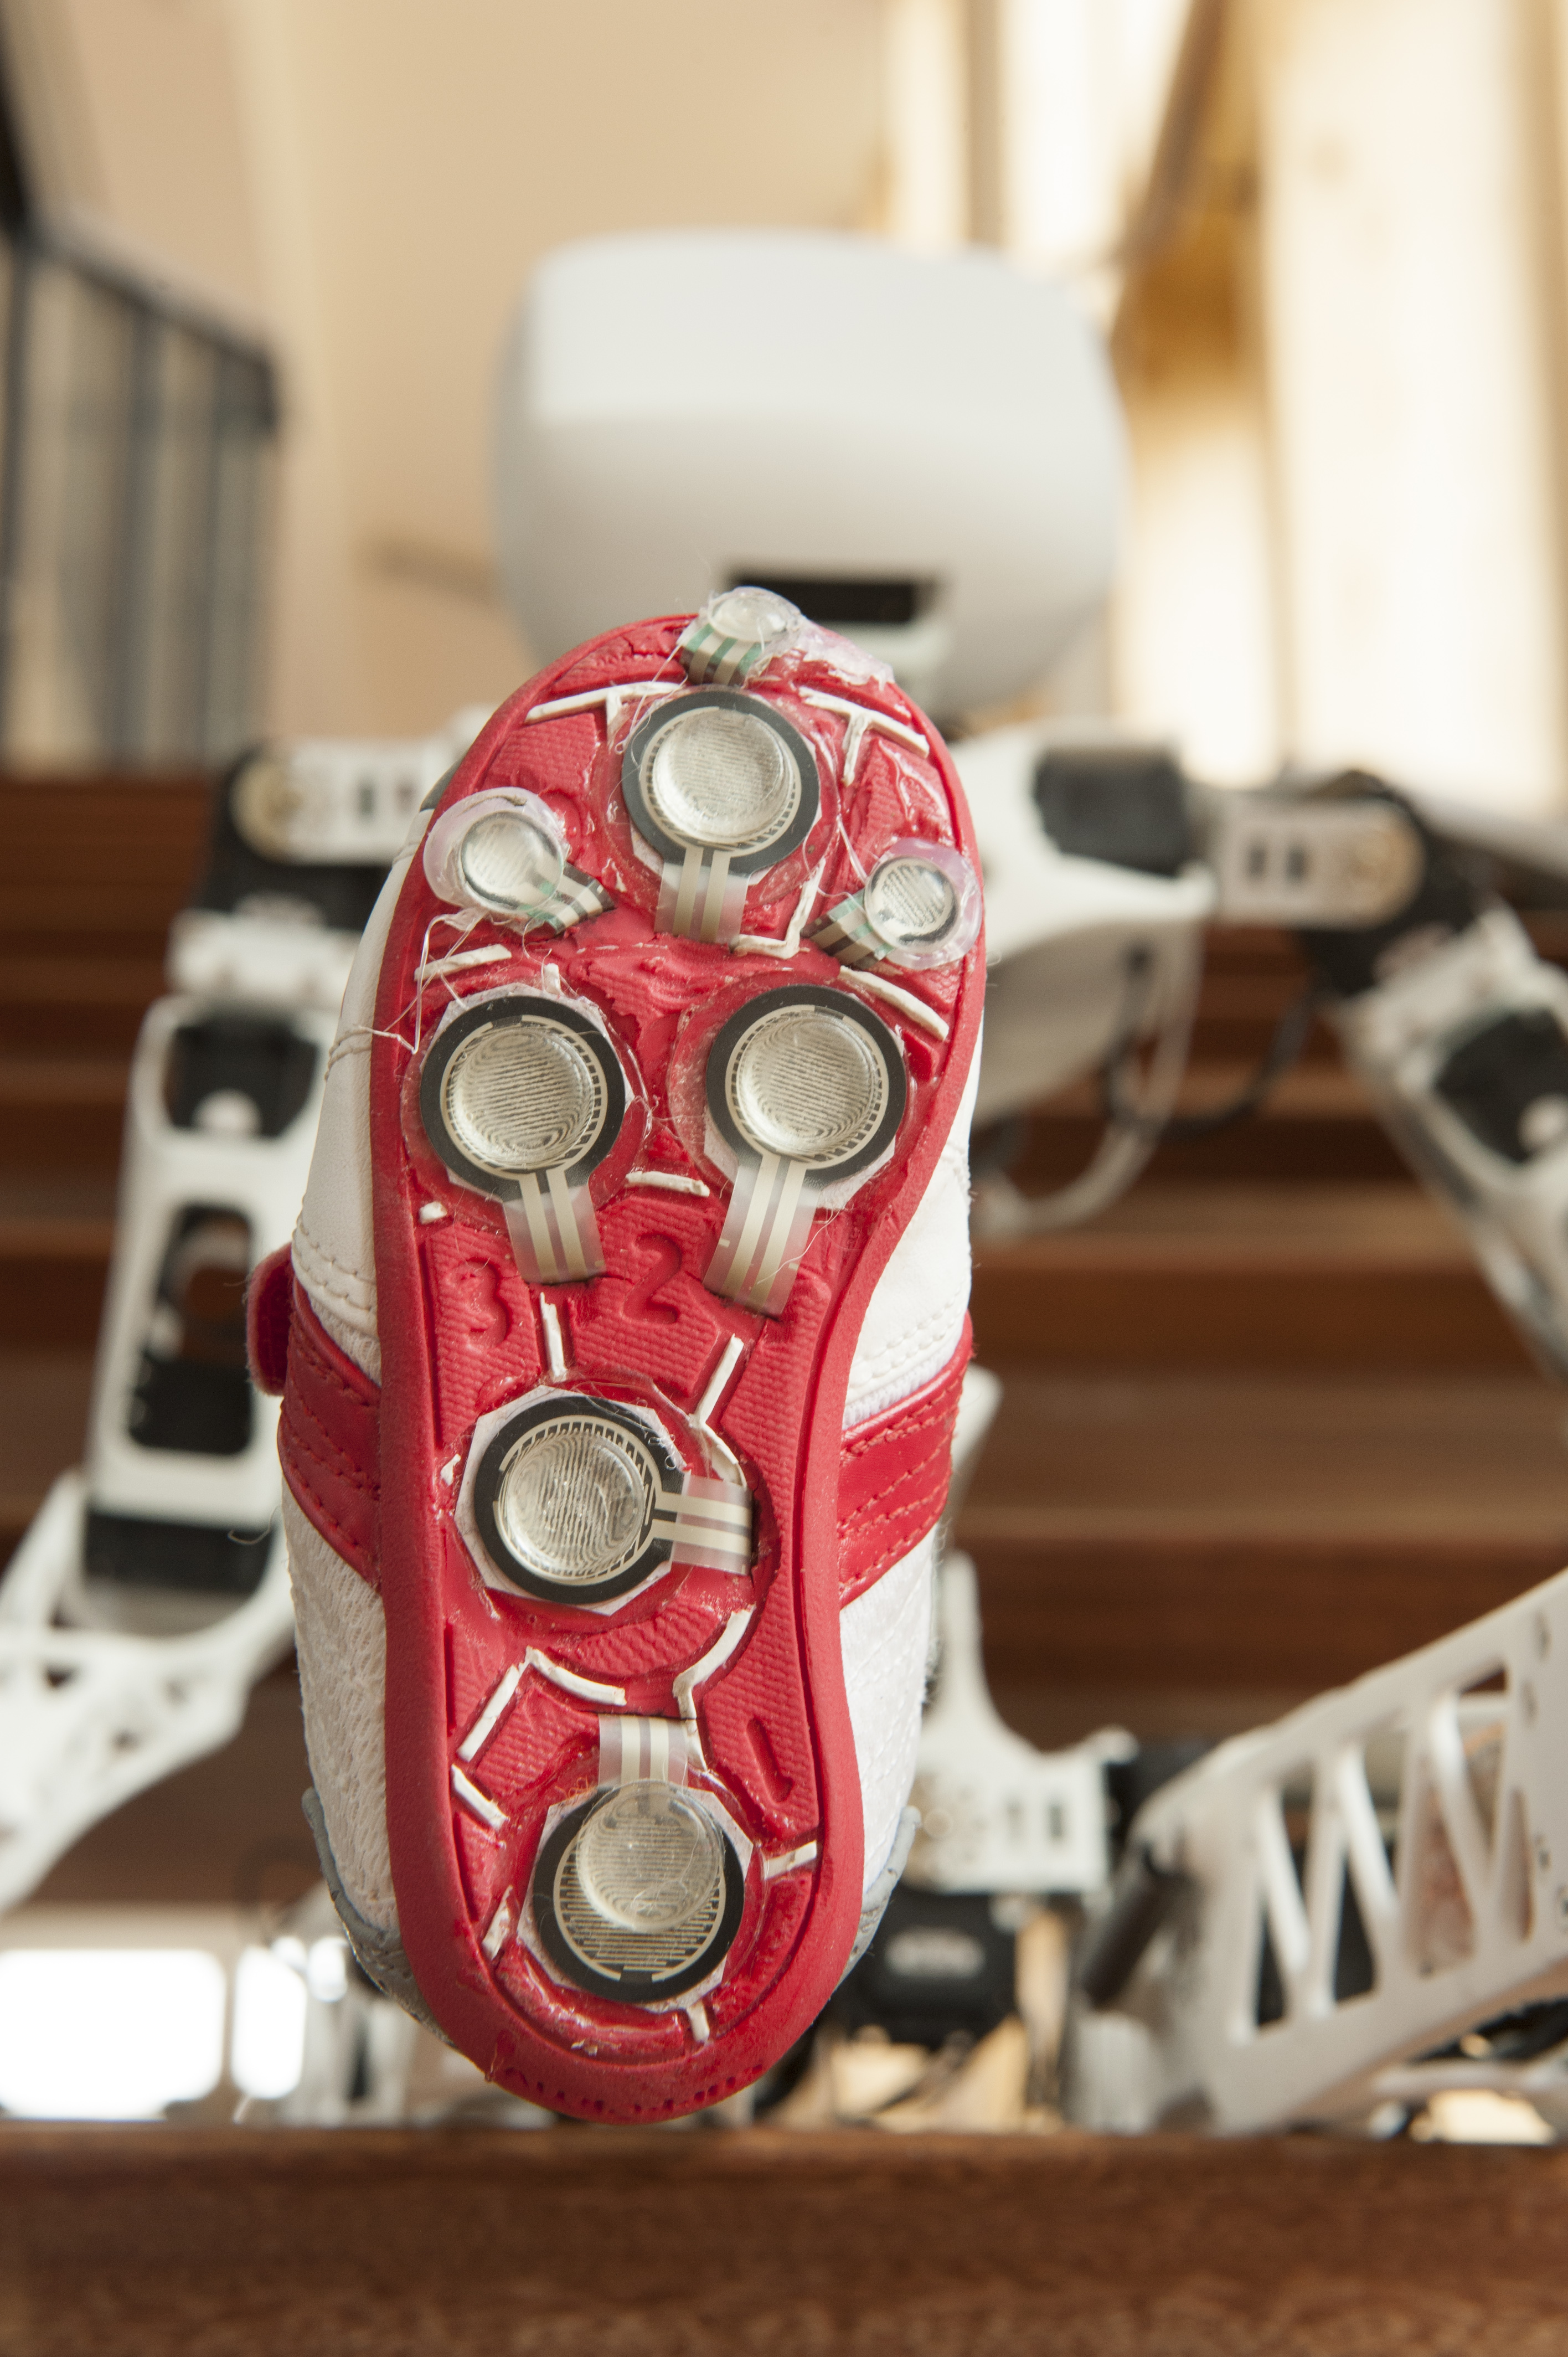
\includegraphics[height=7cm]{foot_sensors.jpg}}
    \hfil
    \subfloat[][]{\label{fig:poppy_nano_integration}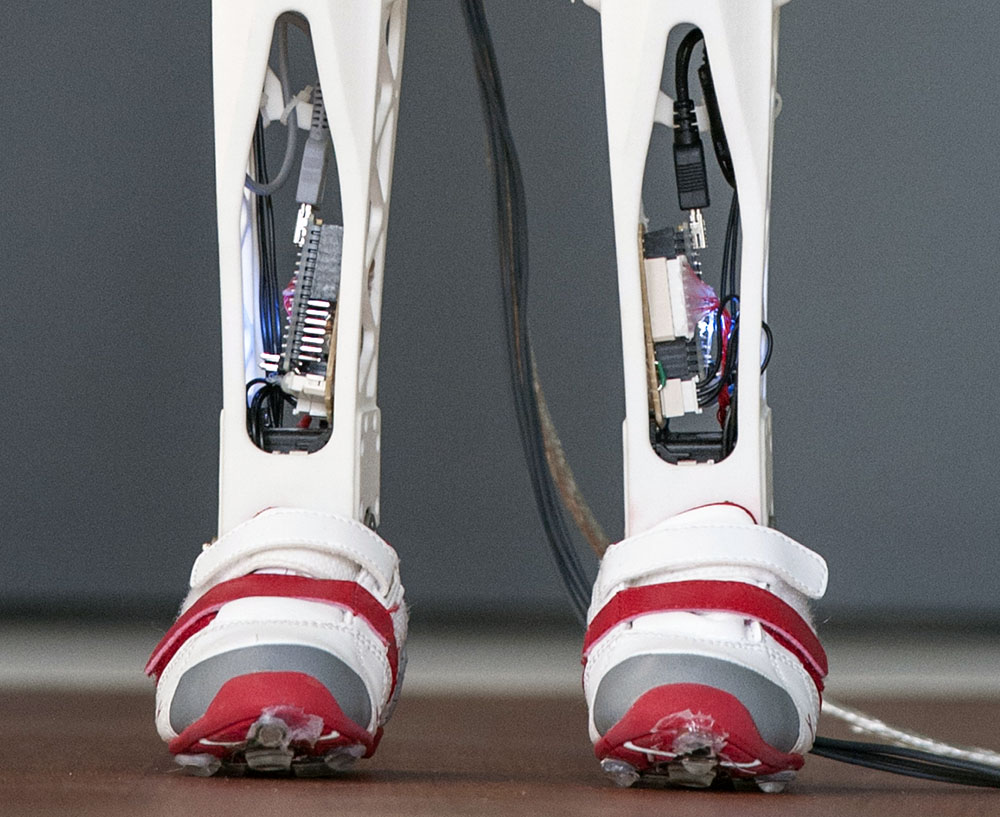
\includegraphics[height=7cm]{poppy_leg_arduino_nano.jpg}}
    \caption{}
    \label{fig:poppy_foot_sensors}
\end{figure}


As we explained in section~\ref{REF}, the Arduino programming language bring the low level programming accessible to anyone. The \codename~\ref{code:arduino_foot_sensor} shows that we actually uploaded on each Arduino nano board. With just 10 lines of code we can stream the values of 5 pressure sensors.

\lstinputlisting[
    language = C++,
    caption = {Arduino code to read force sensors data},
    label = {code:arduino_foot_sensor},
    float,
    floatplacement = H]
    {code/foot_force_sensors.ino}

Then we just have to create a novel sensor controller in pypot (see section~\ref{REF} for details) which describes the I/O communication and get the desired values (see \codename~\ref{code:pypot_foot_sensor}). Here again, the design of the pypot library makes this task easy, only 20 lines of code are required to get access to add a novel sensor and create variable to obtain its value.

\lstinputlisting[
    language = Python,
    caption = {Example of Python code written to add custom foot sensors in pypot. The \emph{FootIO} class describes how we can read the data from the Arduino nano placed in the foot. The \emph{FootPressure} class is the sensor controller which is called by the pypot to synchronize the sensorimotor space of Poppy.},
    label = {code:pypot_foot_sensor},
    float,
    floatplacement = H]
    {code/foot_io.py}


\subsection{Measured data} % (fold)
With our novel sensors, we conducted similar walking experiment as the one explains in section~\ref{REF} and shows on the \figurename~\ref{fig:humanoids2013_cpg_on_poppy} and recorded at $50hz$ the measured force variations under Poppy's feet.

The sensors are not very precise but as we can see on \figurename~\ref{fig:poppy_GRF}, the variation of the ground reaction force (mean of the 5 force sensors) over the gait cycle has a similar M-shape as the one we can find in human gait (see \figurename~\ref{fig:human_GRF}). Also we can notice than the reaction is slightly different between the two foot (\figurename~\ref{fig:right_GRF} Vs \figurename~\ref{fig:left_GRF}).

\begin{figure}[!ht]
\centering
    \subfloat[][]{\label{fig:right_GRF}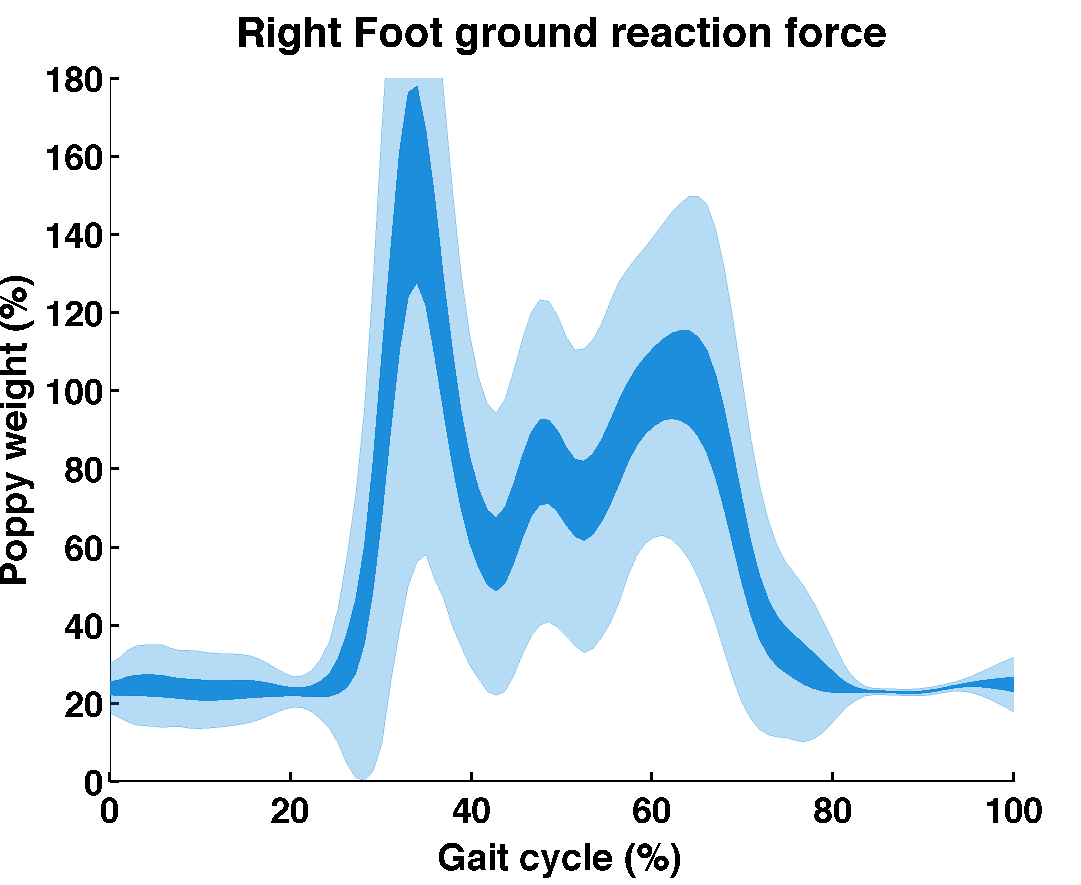
\includegraphics[width=0.48\linewidth]{right_GRF.pdf}}
    \hfil
    \subfloat[][]{\label{fig:left_GRF}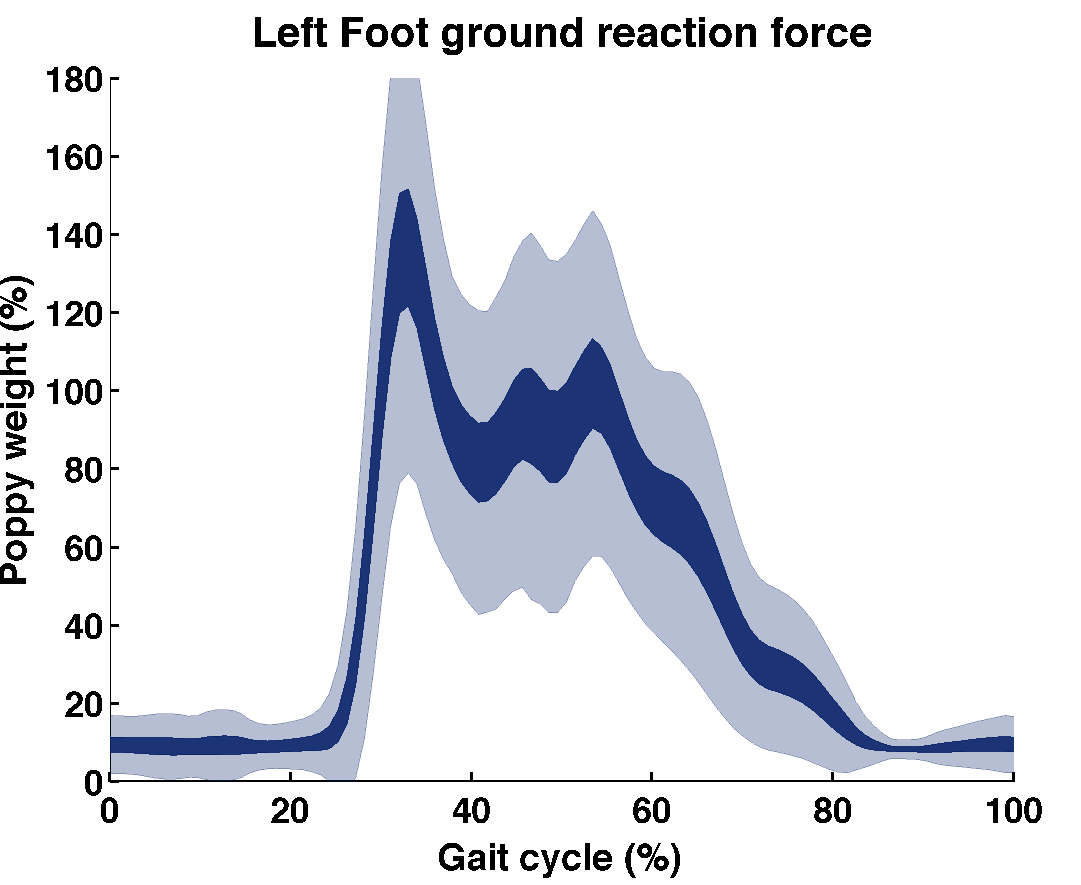
\includegraphics[width=0.48\linewidth]{left_GRF.pdf}}
    \caption{}
    \label{fig:poppy_GRF}
\end{figure}


\begin{figure}[!ht]
\centering
    \subfloat[][]{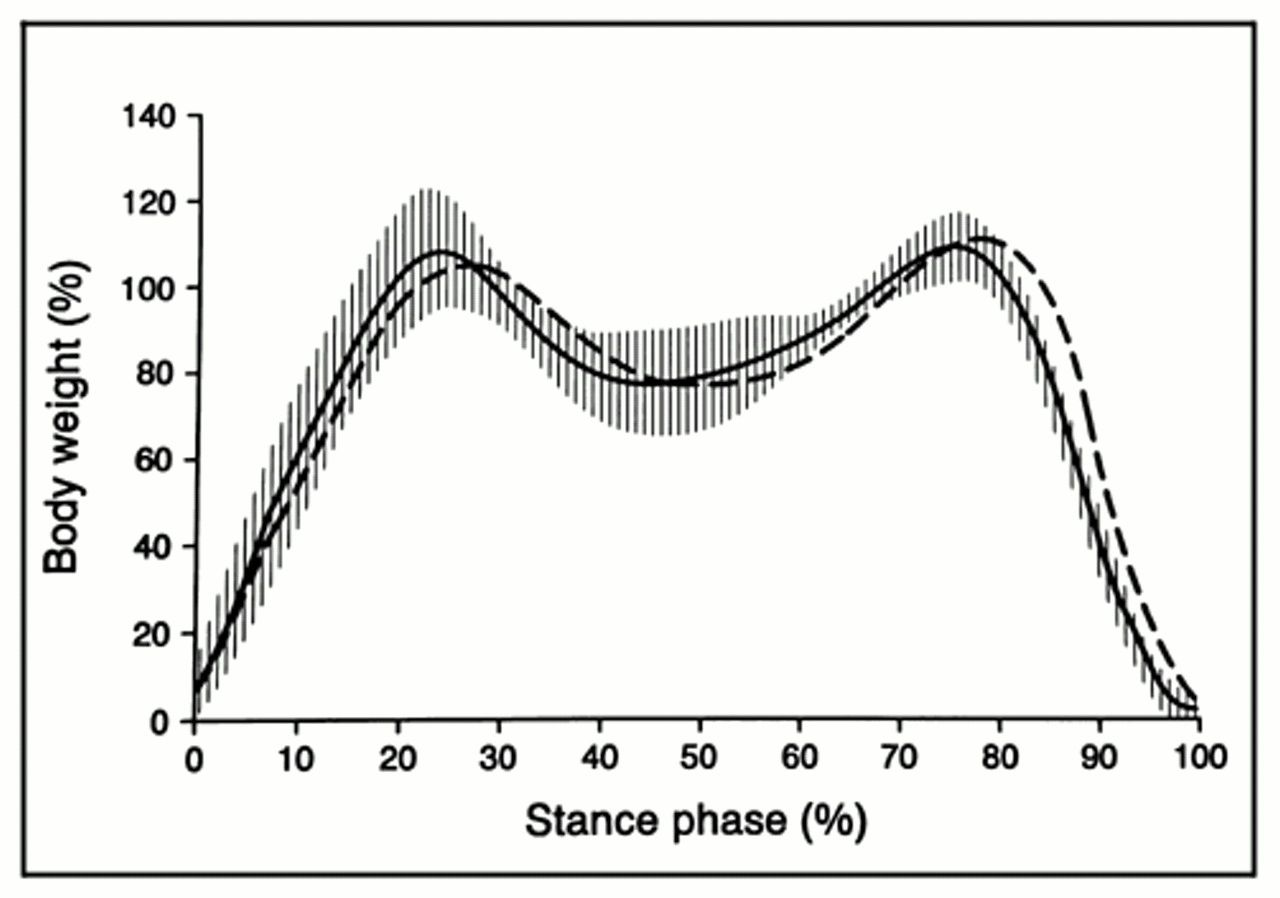
\includegraphics[width=0.3\linewidth]{human_GRF.jpg}}
    \hfil
    \subfloat[][]{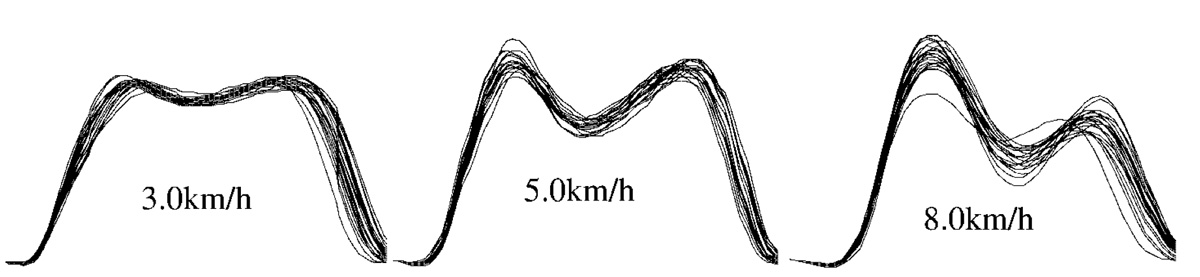
\includegraphics[width=0.7\linewidth]{human_GRF_variation.jpg}}
    \caption{}
    \label{fig:human_GRF}
\end{figure}


The bad precision of the sensors prevents us from affirming conclusions but it can still give insights to understand the walking behavior of Poppy:
\begin{enumerate}
    \item The second peak of the M-shape corresponding to the toe impulsion is weak or inexistent on Poppy. Indeed, when we look at the video of the walking gait made by Poppy, we can notice it barely uses its toes.
    \item The first peak of the M-shape is very strong. Either the walking gait of Poppy was fast or the structure is too rigid and does not absorb correctly the initial impact.
\end{enumerate}

We can therefore explore some improvements axes:
\begin{enumerate}
    \item Explore why the current walking behavior does not involve clearly the passive toes. Is it cause of the walking primitive design or the mechanical design of the toes ?
    \item The initial impact is not desirable toward the achievement of a self-balanced walking behavior. We should explore solutions to absorb it.
\end{enumerate}









\section{Discussion \& Conclusion} % (fold)
\textbf{finding:} Nous avons fait varier plusieur parametres et hacké la platforme de differente manière. Globalement les modifications sont relativements simple à mettre en oeuvre et permettent de rapidement tester de nouvelles morphology à bas coût.
\textbf{conclusion:} Alors ça ouvre la possibilité de
\textbf{ouverture:}
limites il faut quand même le faire à la main, la methode presentée implique de devoir demonter et remonter le robot, même si la tache est rendu le plus simple possible, elle requière une intervention.

Cependant, tout comme l'on peut ajouter des moteurs et des capteurs, on peut très bien imaginer la possibilité de créer des pièces à morphology variable. Cela demande de créer des assemblage adaptés pouvant créer des pièces qui change de dimension.
